\chapter{Substructure Discovery in Tandem Mass Spectometry Data}
\label{c:background}

\section{Introduction}

As the results from Chapter~\ref{c:precursor-clustering} shows, the ionization product (IP) types of many observed peaks are often unknown and therefore the molecular mass of metabolites that generate these peaks are also unknown. This makes identification difficult as mass is often a required information when querying metabolite identities against publicly-available databases, such as KEGG \cite{kotera2012kegg} and PubChem \cite{bolton2008pubchem}. In addition, while modern mass spectrometry instruments can be highly accurate up to 3 parts-per-million (ppm), even a mass accuracy of 1 ppm is not sufficient to reliably determine the elemental composition (formula) of a metabolite \cite{Kind2007} during database queries. The presence of isomers (metabolites having the same formula and mass but are structurally different from each other) suggests that when relying on mass alone, the same peak might be incorrectly matched to multiple isomeric metabolites. Retention time (RT) might help to distinguish certain isomers that have different elution profiles, but RT drift, a main challenge in alignment, means observed RT values can vary across different chromatographic platforms and cannot be easily used as a characteristic information in public databases during identification. Apart from the small number of metabolites present in a standard solution that can be identified with a high degree of confidence (as they produce measured peaks having reliably known m/z and RT values), information on the mass and RT values alone are not enough to establish the identity of many metabolites in untargeted studies. 

Fragmentation spectra are the results of chaining two stages of mass spetrometry steps. In data-dependent acquisition, a precursor or parent (MS1) peak is selected according to a certain criteria, frequently the top-N most intense peaks in a scan, for further fragmentation. This produces for each fragmented parent peak a distinct pattern of fragment (MS2) peaks. Fragmentation patterns can be used to aid identification through the matching of a query spectrum to a database of reference spectra. In recent years, a growing number of fragmentation spectra databases have been made public, including METLIN \cite{Smith2005}, ChemSpider \cite{pence2010chemspider} and MassBank \cite{horai2010massbank}. However, mass spectral databases are not comprehensive and contain only a small number of known metabolites. The large variance in submitted spectra further limits potential matches as sensible results can only be obtained when matching spectra generated from measurement platforms having similar characteristics (for e.g., produced through the same ionization method under a similar mass accuracy). According to \cite{DaSilva2015}, approximately 2\% of spectra in an untargeted metabolomics experiment can be matched and subsequently identified -- a small number in contrast of the vast collection of metabolites that comprise the metabolic pathways of an organism.

Multiple metabolites can share the same chemical substructure. For example, carboxylic acid (Figure~\ref{fig:cooh}) is a generic substructure shared by many amino acids and organic acids. During fragmentation, a characteristic fragment peak 46 Da away from the parent peak --- representing the combined loss of CO and H2O due to the breaking of the neutral carboxyl group (COOH) from the molecular ion --- can be expected to occur in the spectra of metabolites sharing carboxylic acid as a substructure. Knowledge of the constituent substructures that comprise a metabolite, particularly of the larger and more specific substructures, can also be used to provide a hint as to the overall identity of the metabolite. Classification method, such as Support Vector Machine, decision tree and neural networks \cite{Varmuza1996,Hummel2010,Heinonen2012a,Duhrkop2015}, have been trained to learn spectral features that represent substructures and predict the presence or absence of substructures from fragmentation spectra. Combined with information from the parent peak (such as the m/z, RT values and IP types if available), this provides additional information that can aid in the identification of metabolites that cannot be resolved through the traditional method of spectral database matching alone.
\begin{figure}[!htbp]
\centering
\includegraphics[width=0.2\linewidth]{07-lda/figures/927px-Carboxylic-acid.png}
\centering\caption{The carboxylic acid substructure. In the diagram, R refers to the residue, which is the rest of the metabolite attached to this substructure.\label{fig:cooh}}
\end{figure}

A common shortcoming of these classification approaches higlighted before is the need of the supervised training of the classifier (classification-based approaches may fail to generalise well to new dataset produced from different analytical platforms). Based on the assumption that fragmentation spectra contain fragment peaks that represent shared substructures of metabolites, we propose a workflow that applies the Latent Dirichlet Allocation (LDA) model to spectral fragmentation data. The proposed workflow produces the decomposition of fragmentation spectra (equivalently a document in standard LDA) into the set of \textit{Mass2Motifs} (equivalently a topic in standard LDA). Here, a Mass2Motif is defined to be the recurring set of fragment peaks and neutral losses that potentially correspond to a biochemically-relevant substructure shared by many metabolites. Unlike the classification-based methods highlighted earlier, the decomposition of fragmentation spectra into Mass2Motifs is achieved in an unsupervised manner. The MS2LDA workflow is introduced in Section~\ref{sub:ms2lda-workflow}.

\section{Related Work}

Clustering is commonly used for group fragmentation spectra that are similar to each other. Clusters of spectra can be used for identification by forming a consensus spectrum and matching it against spectral databases. Molecular networking clusters MS1 peaks by their MS2 spectral similarity such that one identifiable metabolite in a cluster facilitates structural annotation of its neighbors \cite{yang2013molecular, nguyen2013ms, van2016urinary}.  However, only MS2 spectra with high overall (e.g. cosine) spectral similarity are grouped in Molecular Networking. Consequently Molecular Networking may fail to group molecules that share small substructures. In particular, spectra may be placed in different clusters if they share a small number of fragment peaks that related to a common substruture, but their overall global similarities are too different. Even for spectra placed into the same cluster, often manual analysis (by eyes) is required to select the characteristic fragment peaks that represent a potential substructure and are shared by members of the clusters. Another package, MS2Analyzer \cite{ma2014ms2analyzer} mines MS2 spectra given the prior knowledge on the fragment patterns of interest to be specified in advance. While generic features, such as CO or H2O losses, will be common to many experiments, sample-specific features can be easily overlooked if they have not been specified \textit{a priori}.

The assumption that spectral consist of building blocks that correspond to substructures is alluded in certain works but not directly mined from the data. Prior knowledge on substructures have been used for the annotations of a small number of moelcules in fragmentation data \cite{Sweeney2014} and for metabolite classification in GC-MS \cite{Scott1994, Hummel2010}. In CSI:FingerID \cite{Duhrkop2015}, a fragmentation tree is used to predict (using Support Vector Machine) the molecular `fingerprint', computed through the implicit assumption that fragments share substructures, of an unknown compound. The resulting fingerprint is used to improve the matching of spectrum of the unknown compound against a vast chemical database (PubChem). Implicit in these methods are the assumption that recurring patterns of fragment peaks and neutral losses values explain the presence of common biological substructures (e.g. a hexose unit, or a CO loss) shared by metabolites. 

Latent Dirichlet Allocation has not been applied to metabolomics or mass spectrometry data, but it has been applied to other fields of computational biology in e.g. genomics \cite{chen2010probabilistic}, metagenomics \cite{zhang2015exploiting}, and transcriptomics \cite{rogers2005latent}. In \cite{chen2010probabilistic}, DNA sequence from genomics studies is decomposed into recurring patterns of N-mers nucleotides. A topic in this context corresponds to the set of N-mers (e.g. `ATGC' as an instance of a 4-mers) that co-occur together across the different genomic sequences of a species, and the objective of the study is characterise the sets of N-mers that corresponds to conserved genes of the species. Similarly in \cite{zhang2015exploiting}, a metagenomic read (essentially a DNA sequence) is decomposed into its topic distribution. The unsupervised decomposition of metagenomic reads into topic distributions is used to improve the binning (clustering) of reads from the same species. In \cite{rogers2005latent}, a sample or gene from transcriptomics studies is decomposed into multiple processes in a manner similar to how a document is decomposed into different topics in traditional LDA for text.

\section{Statement of Original Work}

The work discussed in this chapter has been submitted to the \textit{Proceedings of the National Academy of Sciences} and is under review. Justin van der Hooft (JvdH) performed the measurements of the Beer samples through mass spectometry, generating the set of fragmentation data that can be used for topic modelling. The author contributed to the design and development of the MS2LDA workflow. This includes the development and optimisation of the feature extraction process, the implementation and testing of inference via LDA and also model validation against multinomial mixture model. 

JvdH then analysed the results from MS2LDA for biochemical significance. To assist JvdH in his analysis, the author proposed and developed the visualisation module, MS2LDAVis. To improve the visualisation module, the author integrated elemental formula annotation functionalities. This includes writing a wrapper in MS2LDA to call SIRIUS \cite{Bocker2009}, a Java-based elemental formula annotator. Cristina Mihailescu (CM) implemented another Python-based elemental formula annotator, which was also customised and integrated into MS2LDA by the author. 

JvdH then performed molecular networking analysis on the same dataset, which was used for comparison to MS2LDA results. The author performed the identification of metabolites through matching to reference standard compounds and also the differential analysis of Mass2Motifs, and JvdH validated the results. 

\section{A Workflow for Substructure Discoveries and Annotations\label{sub:ms2lda-workflow}}

Substructure discovery through the MS2LDA workflow consists of two stages: i) the data conversion stage, which prepares the acquired fragmentation data into suitable input format for the workflow, followed by ii) the Mass2Motif discovery stage, which performs topic modelling via LDA to discover mass fragmental patterns, assigns potential candidate elemental formulae to MS1 and MS2 peaks, and visualises the Mass2Motifs in an interactive environment. The key insight of MS2LDA lies in emphasising the parallel between text and mass spectrometry fragmentation data (Figure~\ref{fig:text2frags}A-B). As a text analysis pipeline relying on LDA to decompose documents into topics based on frequently co-occurring words, so MS2LDA decomposes fragmentation spectra into their constituent building blocks of frequently co-occurring fragments and neutral losses (referred to as ‘Mass2Motifs’). The complete workflow is illustrated in Figure~\ref{fig:text2frags}C. 

\begin{figure}[!htbp]
\centering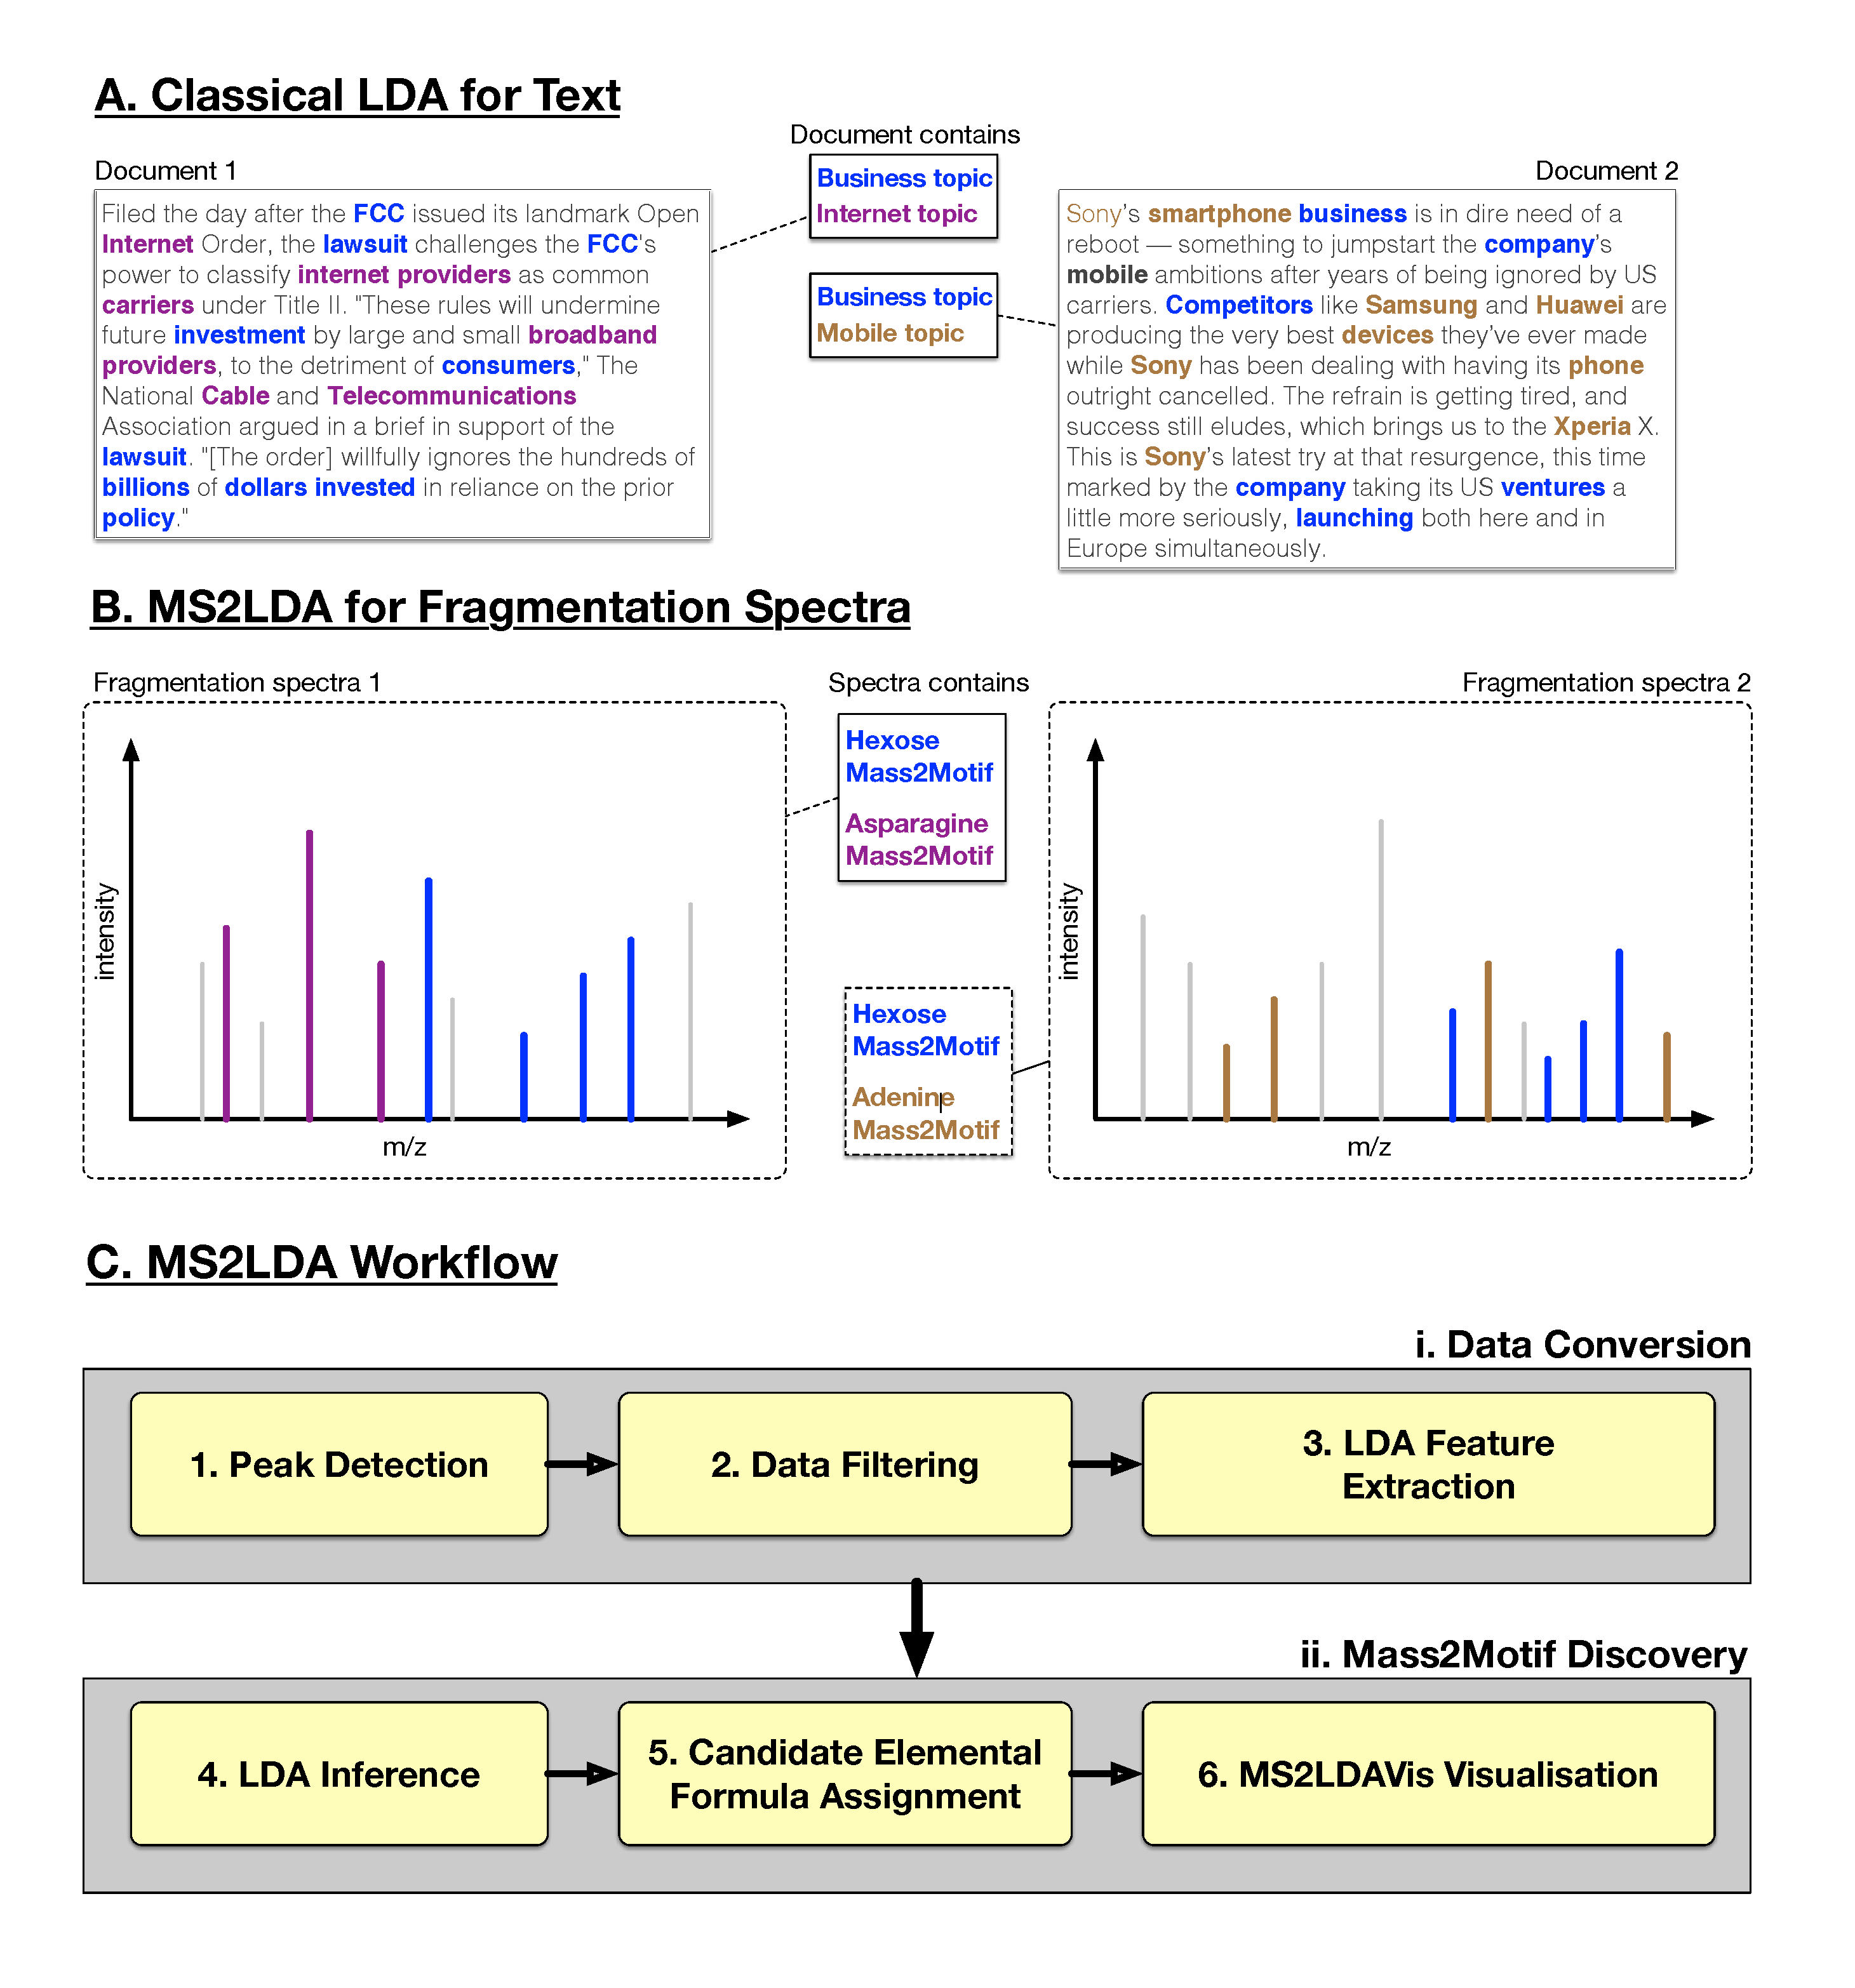
\includegraphics[width=1.0\linewidth]{07-lda/figures/text2frags_new.pdf}
\centering\caption{\textbf{A.} LDA applied to text decomposes a document into its topic distributions (e.g. football, business and enrivonment topics). \textbf{B.} Similarly, MS2LDA decomposes a fragmentation spectrum into its topics (Mass2Motifs) that can be characterised as asparagine, hexose and adenine related. Each fragmentation spectra comprise of one or more Mass2Motifs. \textbf{C.} Schematic overview of the MS2LDA workflow.\label{fig:text2frags}}
\end{figure}

Acquired fragmentation data cannot readily be used for the purpose of pattern searching via LDA and has to be converted into a suitable format. As input, the MS2LDA workflow accepts the combination of a single full-scan file for the MS1 peaks and a separate fragmentation file for the MS2 peaks. The data conversion process starts with the detection of MS1 peak in the input .mzXML file obtained from full-scan mode spectra using the CentWave algorithm from the XCMS library \cite{Smith2006}. This constitutes information on the parent (MS1) level. Fragmentation data, in the form of .mzML file obtained from tandem MS mode, are processed using an R script based on the RMassBank package \cite{Stravs2013}. 

A linking step is required to match the most intense MS2 spectrum in a scan to a parent MS1 peak. Matching is performed via a greedy search within a specified retention time tolerance window, selecting the top few most intense peaks for the matching. This simulates the generative process that produces the spectral data in data-dependant experiments. A filtering step, based on RT and intensity, is applied to remove noisy peaks. Any MS1 peak not having paired MS2 peaks is also discarded for further processing. The aim of the filtering step is to exclude identical fragmentation spectra produced by low-intensity MS1 peaks that were fragmented multiple times, potentially forming spurious and uninformative Mass2Motifs on their own. 

Following the bag-of-words assumption, LDA does not consider word orders but instead take into account only the number of times word co-occur in a document. The next step is transforming spectral data into a bag-of-word count matrix (illustrated in Figure~\ref{fig:m2lda-matrix}), with entries in the matrix the co-occurrences of discrete MS2 features (`words') in the fragmentation spectra linked to a parent MS1 peak (`document'). From each fragmentation spectra, two types of features can be extracted: fragment features and loss features. Fragment features are the discretised m/z values of MS2 peaks, while loss features are formed by discretising neutral losses. A neutral loss, defined as the mass differences between a precursor MS1 peak and each of the child MS2 peaks in the spectrum, corresponds to the removal of a specific neutral fragment from the molecular ion. 

\begin{figure}[!htbp]
\centering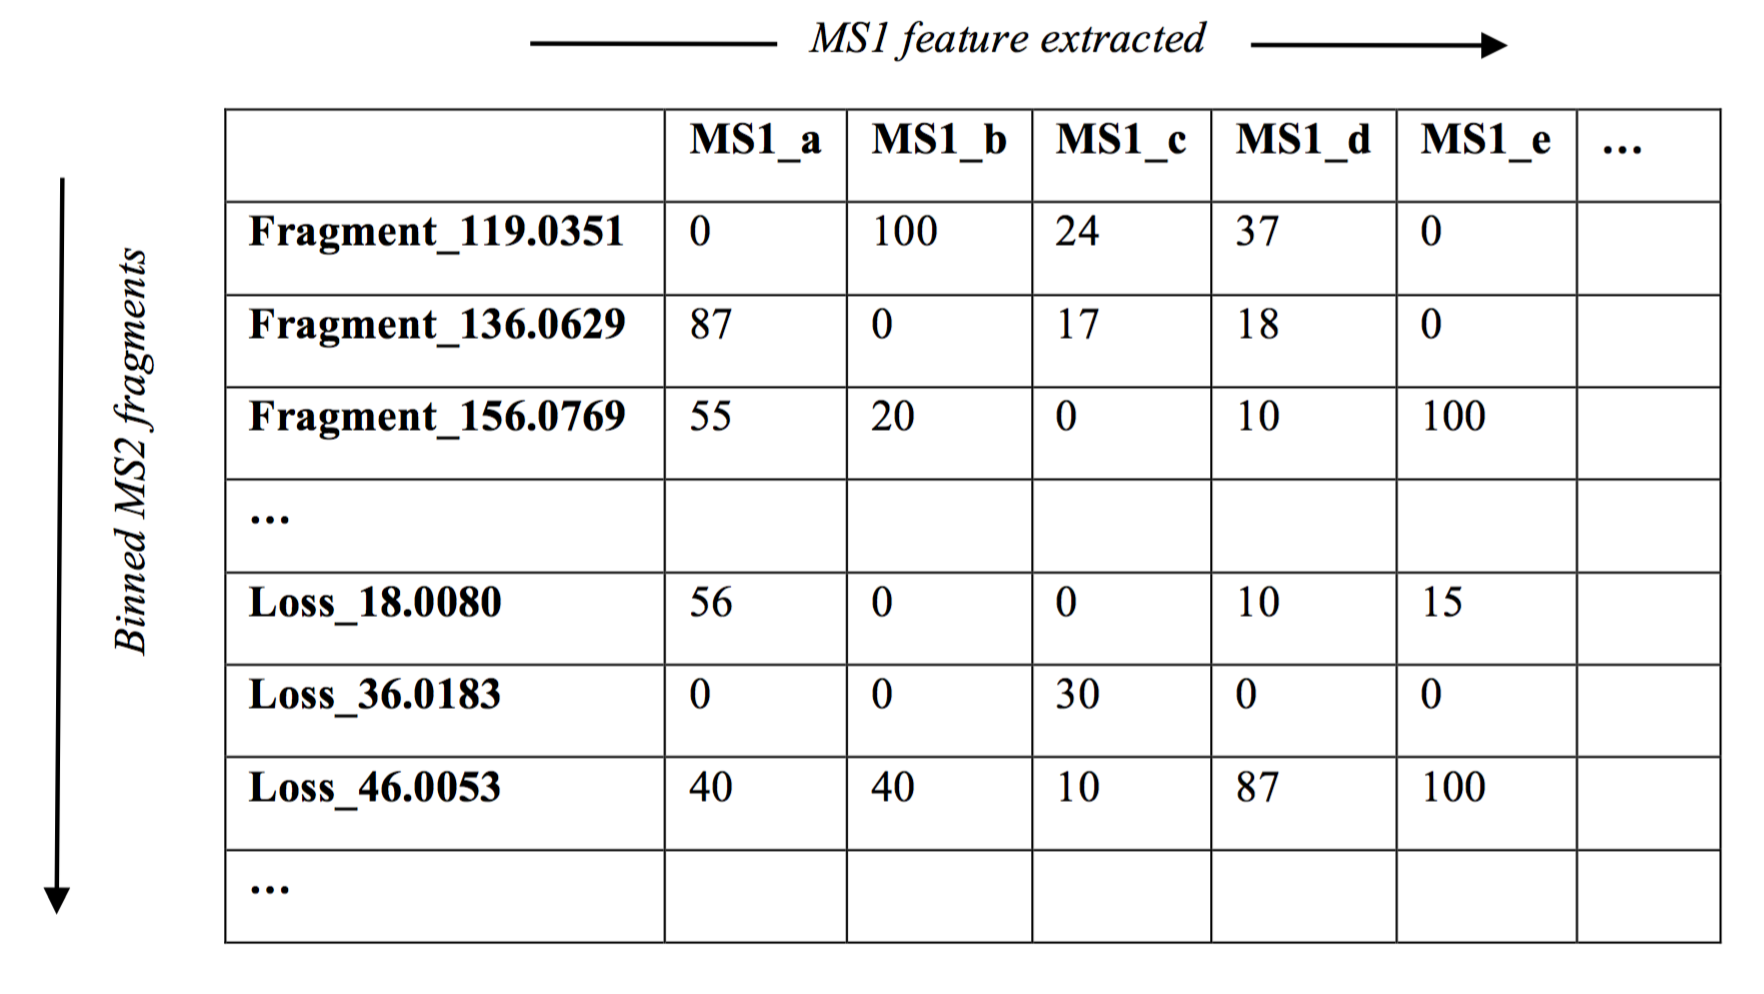
\includegraphics[width=0.8\linewidth]{07-lda/figures/matrix.png}
\centering\caption{The matrix of co-occurrences of fragment and loss features (rows) in each fragmentation spectrum linked to a parent MS1 peak (columns). Entries of the matrix are the counts of the feature from the normalized (0 – 100 scale) intensities.\label{fig:m2lda-matrix}}
\end{figure}

Discretisation is performed via a greedy binning process. To group continuous m/z values and create fragment features, a priority queue is used that efficiently maintains the ordering of m/z values of peaks upon insertion. Successive items are popped from the priority queue in ascending order, forming a group of contiguous features --- until the next encountered item has an m/z value larger by a predefined tolerance in parts-per-million from the average values of the group, in which case a new group is created. The average m/z values of a group, rounded to 5 decimal places, becomes the discrete representation of fragment peaks in their originating spectra. The count of a fragment feature in a spectrum is computed by dividing the MS2 peak's intensity value to the largest intensity in the spectrum and multiplying by an scaling factor of 100 (equivalent to the discretisation resolution). In this manner, MS2 peaks with larger intensity values are represented more often in the spectra. Neutral loss features are discretised and computed in a manner similar to fragment features. The resulting matrices for fragment and loss features are concatenated and used as input to LDA. % Another possible informative feature considered but yet unused in MS2LDA is the pairwise differences between all MS2 peaks in a spectrum, which represent the potential substructures broken off from the original compound during fragmentation.

In the context of fragmentation data, the standard LDA model as applied to substructure discovery is described next. The observation on the $n$-th fragment or loss feature in the $d$-th fragmentation spectra ($w_{dn}$) is conditioned on the assignment of feature $w_{dn}$ to the $k$-th Mass2Motif multinomial distribution. This corresponds to the topic distribution over words in the original LDA model. This assignment is denoted by the indicator variable $z_{dn}$, so $z_{dn}=k$ if feature $w_{dn}$ is assigned to a $k$-th Mass2Motif. The $k$-th multinomial distribution that a feature is assigned to is characterised by the parameter vector $\boldsymbol{\phi}_{z_{dn}}$, with $\boldsymbol{\phi}_{z_{dn}}$ drawn from a prior Dirichlet distribution with a symmetric parameter $\beta$. 
\begin{align}
w_{dn} \vert \boldsymbol{\phi}_{z_{dn}} &\sim Multinomial(\boldsymbol{\phi}_{z_{dn}}) \\
\boldsymbol{\phi}_{k} \vert \beta &\sim Dirichlet(\beta)
\end{align}
The probability of seeing certain Mass2Motifs for each $d$-th fragmentation spectra is drawn from a multinomial distribution with a parameter vector $\boldsymbol{\theta}_{d}$, corresponding to the topic decomposition of a document in the original LDA model. This parameter vector $\boldsymbol{\theta}_{d}$ is in turn drawn from a prior Dirichlet distribution having a symmetric parameter $\alpha$. 
\begin{align}
z_{dn} \vert \boldsymbol{\theta}_{d} &\sim Multinomial(\boldsymbol{\theta}_{d}) \\
\boldsymbol{\theta}_{d} \vert \alpha &\sim Dirichlet(\alpha)
\end{align}
A collapsed Gibbs sampling scheme is implemented in Python for inference (details in Section~\ref{background-lda}). The output from inference is a set of Mass2Motifs and assignments of Mass2Motifs to each MS1 peak. 

\subsubsection{MS2LDAVis}

% \textbf{(the visualiser was all your idea!…it doesn’t get much mention in the chapter actually…).}

Given its hypothesis-generating nature, the analysis of Mass2Motifs to characterise and examine their correspondence to actual biochemical substructures is an iterative and exploratory process. This is made possible through the MS2LDAVis module, an interactive web-based visualisation build upon the combination of the Javascript and the D3 library (http://d3js.org). MS2LDAVis is extended from the Python port of the topic modelling visualisation interface LDAVis \cite{Sievert2014} used in the text domain, but our adaptation MS2LDAVis introduces fragmentation-specific views.

\begin{figure}[!htbp]
\centering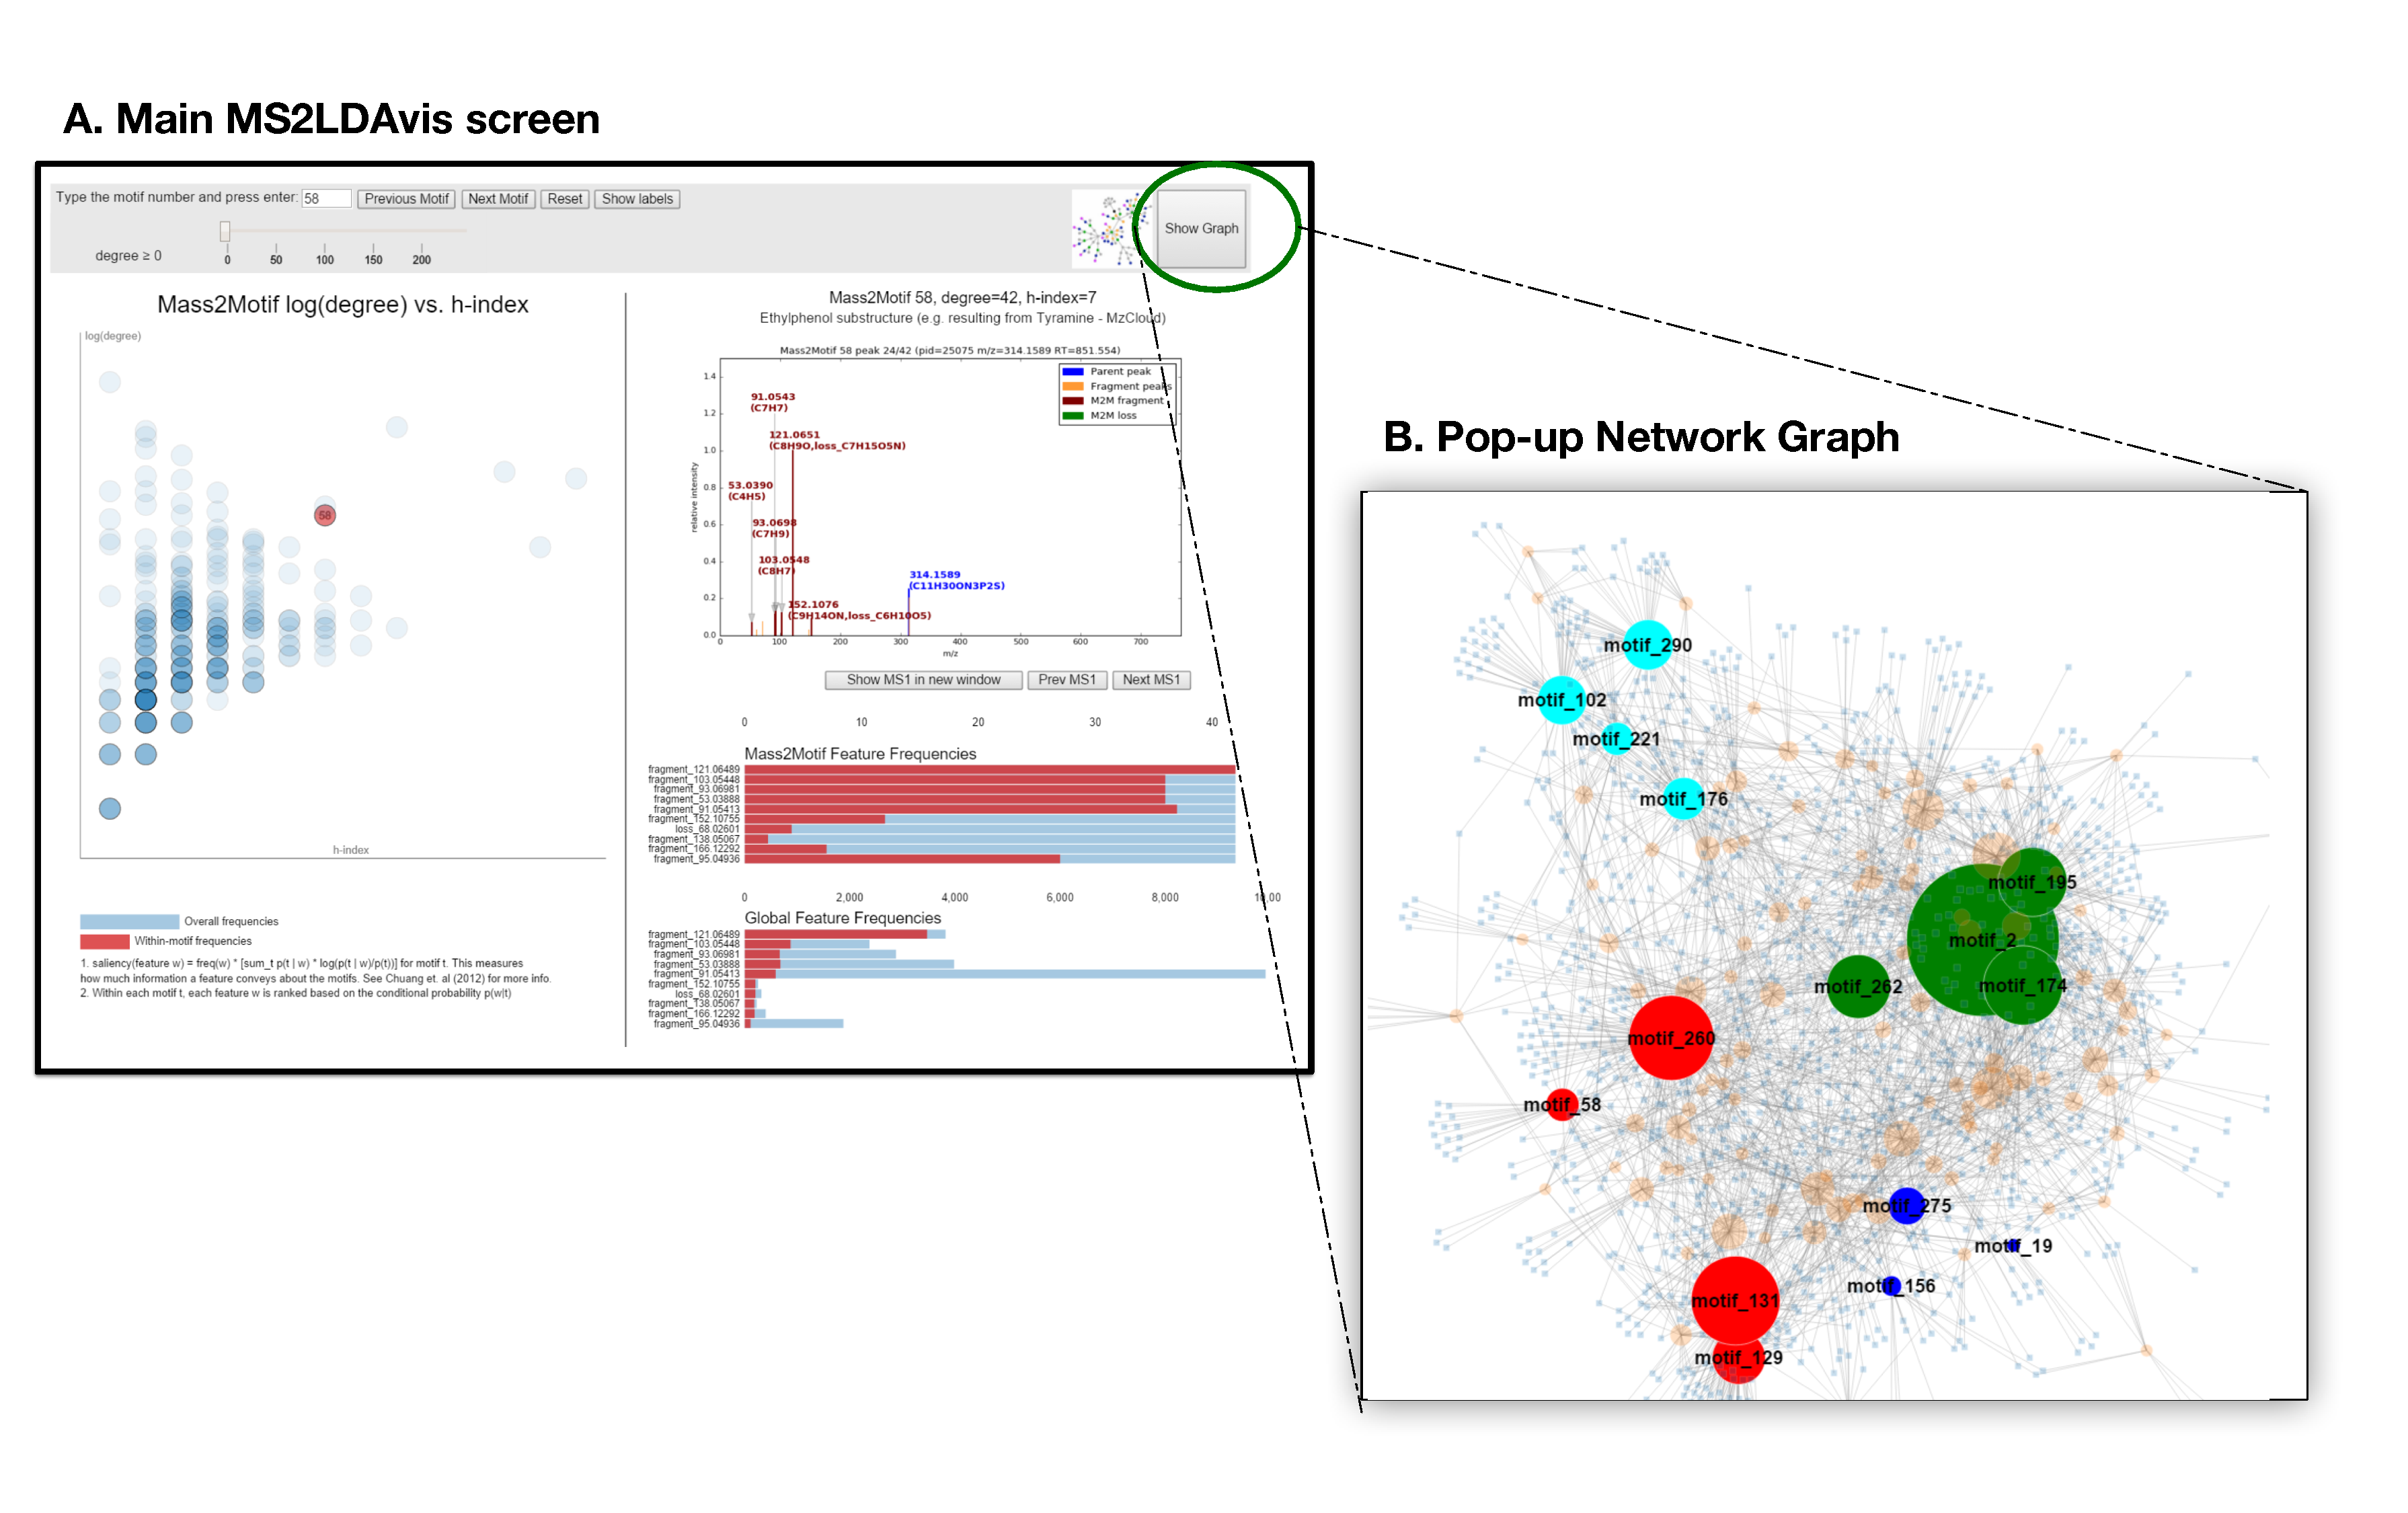
\includegraphics[width=1.0\linewidth]{07-lda/figures/figure_s3.pdf}
\centering\caption{Screenshot of MS2LDAVis. See text for explanations of the different panels.\label{fig:m2ldavis-main}}
\end{figure}

Similar to the original LDAVis, the left panel of MS2LDAVis module shows a global view of the model, whilst the right panel zooms into a specific Mass2Motif (see Figure~\ref{fig:m2ldavis-main}A). However, unlike LDAVis where topics are displayed on the left panel through multidimensional scaling that projects topics to two dimensions, the two axes in MS2LDAVis panel are the log-degree and the $h$-index of Mass2Motifs. The degree of a Mass2Motif as the number of fragmentation spectra explained by the Mass2Motif at the user-defined threshold $t_{\theta}$ on the fragmentation-spectra-to-Mass2Motif distributions ($\boldsymbol{\theta}$). The $h$-index of a Mass2Motif is defined in a similar manner to the conventional $h$-index for scientific publications of a researcher. A Mass2Motif has an index of $h$ if it has $h$ fragment or loss features obtained after setting a user-defined threshold $t_{\phi}$ on the Mass2Motif-to-features distributions ($\boldsymbol{\phi}$), each of which occur in the set of thresholded spectra at least $h$ times. Intuitively, a Mass2Motif with high degree but low $h$-index may potentially correspond to simple substructures that occur in many fragmentation spectra, while a Mass2Motif with high $h$-index but low degree are more unique and complex substructures shared by fewer MS2 spectra.

Selecting a Mass2Motif on the left panel of Figure~\ref{fig:m2ldavis-main}A changes the specific information displayed on the right panel. Fragmentation spectra that can be explained by the currently selected Mass2Motif (above the threshold $t_{\theta}$) are plotted, and clicking the ‘Previous MS1’ and ‘Next MS1’ buttons allows the flipping through consecutive spectra plots. Fragment and loss features that can be explained by the selected Mass2Motif (above the threshold $t_{\phi}$) that also occur in the plotted spectra are highlighted in bold. Two barplots can be found on the bottom right panel: the Mass2Motif Feature Frequencies displays the counts of each fragment or loss features within the entire fragmentation spectra explained by the currently selected Mass2Motif, while the Global Feature Frequencies displays the counts of the fragments or loss features within the complete data set that can be explained by the currently selected Mass2Motif.

To complement the main visualisation view, inference results can also be visualised in a pop-up network graph (Figure~\ref{fig:m2ldavis-main}B) by clicking the ‘Show Graph’ button. In the network view, Mass2Motifs and fragmentation spectra, represented by their parent MS1 peaks in the graph, form the nodes in the graph, and edges are drawn between the nodes if a spectra can be explained by a Mass2Motif above the threshold $t_{\theta}$. To minimise clutter in the graph, a slider is provided to filter nodes based on their degree values. Nodes in the graph can also be annotated and coloured according to user specifications before the visualisation interface is called. The two complementary views are linked such that clicking a Mass2Motif node on the network graph will select the corresponding Mass2Motif on the main view and vice versa. The network graph is particularly useful in exploring the relationships between Mass2Motifs and investigating which spectra can be explained by multiple Mass2Motifs.

To aid data interpretation, putative elemental formulae is displayed on the plots of fragmentation spectra explained by a certain Mass2Motif (top-right panel, Figure~\ref{fig:m2ldavis-main}). Two methods are integrated within MS2LDA to assign candidate elemental formulae. SIRIUS \cite{Bocker2009} employs a dynamic programming approach, termed `Round Robin' \cite{Bocker2007}, to solve elemental formula assignment as an integer decomposition problem. SIRIUS is freely-available and, as it is written in Java, can in theory be run platform-independently on any Windows, Unix and Mac environment (in practice, library dependencies have to be satisfied before SIRIUS can run). Integration of SIRIUS into the MS2LDA workflow is achieved by wrapping calls to the Java classes of SIRIUS through a separate sub-process, passing it a temporary MGF file that corresponds to a fragmentation tree. SIRIUS assigns elemental formulae to each fragmentation tree independently, which may lead to mass fragments of similar m/z value being assigned an elemental formula in some spectra, but not in all.

As an alternative to elemental formula annotation via SIRIUS, CM developed EF-Assigner, a pure Python implementation of an elemental formula assigner based on the Round Robin algorithm on which SIRIUS is based on. In EF-Assigner, candidate formulae are filtered using an implementation of the 7-golden rules, a set of heuristic rules introduced in \cite{Kind2007} to remove chemically-unlikely elemental formula compositions from the candidate list. The advantages of EF-Assigner are its easy integration with the rest of the workflow (it is also written in Python) and it can assign elemental formulae to an entire group of MS2 peaks as represented by their discrete fragment and loss features at once. Unlike SIRIUS that uses the complete information of the precursor ion and fragments peaks in a spectrum for annotation, EF-Assigner assigns the elemental formulae for the MS1 peaks and MS2 fragment and loss features independently. The author included EF-Assigner in the MS2LDA workflow, passing it the necessary MS1 peaks and MS2 fragment and loss features for annotation. EF-Assigner is also modified to limit the maximum atom occurrences of certain elements in a candidate formula. For a greater annotation coverage, a second stage process is implemented. After an initial pass of EF-Assigner using a list of common chemical elements of CHNOPS, unannotated MS1 peaks and MS2 features are then re-annotated using an expanded list of possible elements that includes less common elements, such as the C-13 isotope of Carbon, Fluorine and Chlorine.

\section{Evaluation Study}

\subsection{Evaluation Dataset\label{sub:ms2lda-datasets}}

To evaluate MS2LDA, four beer samples representative of complex mixtures of diverse biochemically relevant compound classes (such as amino acids, nucleotides, and sugars) typical in metabolomics studies are used. The beer extracts, acquired from one home-brewed beer and three different commercially available beers, are shown in Table~\ref{tab:beer-sample-details}. One of the beer samples (Beer3) is also used for the evaluation of the alignment methods in Chapter~\ref{c:matching}. Approximately 10 ml of beer was sampled from each bottle directly after opening. As well as the four individual extracts, a pooled aliquot of the four beer extracts was prepared. A Thermo Scientific Ultimate 3000 RSLCnano liquid chromatography system, coupled to a Thermo Scientific Q-Exactive Orbitrap mass spectrometer comprise the overall LC-MS setup.

Following mass spectrometry, blank runs, quality control samples, and 3 standard mixes containing 150 reference compounds were run to assess the quality of the mass spectrometer and aid in metabolite annotation and identification \cite{Creek2011}. The pooled sample was run prior to and across the batch to monitor the stability and quality of the LC-MS runs. Beer samples were run in a randomized order. Immediately after acquisition, all RAW files containing information stored in a proprietary vendor-dependant format were converted into the open mzXML format. Mass spectra are centroided and separated into positive and negative ionization modes using the command line version of MSconvert (ProteoWizard). Fragmentation files were also converted into .mzML formats using the GUI version of MSconvert.  Accurate masses of standards were obtained well within 3 ppm accuracy and intensities of the quality control samples (a beer extract and a serum extract) were as expected. 

\begin{table}[!htbp]
\small
\centering
\begin{tabular}{|l|l|}
\hline
\textbf{Label} & \textbf{Source}                                                                                                                                                                                        \\ \hline
Beer1          & A home-brewed bottle of German Wheat Beer. \\ \hline
Beer2          & A bottle of `Jaw Glyde Ale’ brewed by JAW Brew. \\ \hline
Beer3          & A bottle of `Seven Giraffes Extraordinary Ale’ brewed by William Bros. Brewery Company. \\ \hline
Beer4          & A bottle of `Black Sheep Ale’ brewed by Black Sheep Brewery. \\ \hline
\end{tabular}
\caption{Beer samples used for evaluation dataset.}
\label{tab:beer-sample-details}
\end{table}

\subsection{Model Comparison}

We performed model selection via a 4-folds cross validation approach on one of the data file (Beer3 positive ionization mode). For each test fold being held out in the Beer3 data file, an estimate of the model evidence is computed after training the model on the remaining training folds in the file. The number of Mass2Motifs was also selected in this manner from cross-validation. 

A crucial difference between LDA and the multinomial mixture-model (clustering) lies in the modelling assumption that a document is a mixture of one or more topics (LDA) as opposed to each document having exactly one topic (clustering). To validate one of our key assumptions of Mass2Motifs represent biological building blocks (i.e. fragmentation spectrum contains more than one Mass2Motifs), we compared the LDA model to a multinomial mixture model that can also be used for the clustering of fragmentation spectra. A comparison of LDA to a multinomial mixture model was performed by the author to assess and validate model fit, evaluated based on perplexity on the held-out data. Perplexity measures how well a probability distribution or probability model predicts a sample and is defined as:
\begin{align*}
perplexity(W)=exp\left(\frac{\sum_{d}log(P(w_{d})}{\sum_{d}N_d}\right)
\end{align*}
where $perplexity(W)$ is the perplexity on the whole held-out test collection, $P(w_d)$ is the marginal probability of a testing spectra $d$ (integrating over all the parameters of the model), approximated via an importance sampling method \cite{wallach2009evaluation} and $N_d$ is the number of features in each testing spectra $d$. Following \cite{Griffiths2004}, the hyper-parameters were set to $\alpha=K/50$ and $\beta=0.1$ during cross-validation. For mixture model clustering, a non-informative Dirichlet prior ($\alpha=K/50$, where $K$ is now the number of clusters) is set on the proportions of the mixture components and another Dirichlet prior ($\beta=0.1$) is set on cluster-specific word distributions. The Gibbs sampler for LDA and multinomial mixture model is run for 1000 samples, discarding the first 500 for burn-in. The last sample is used computing the posterior estimates. Minimal differences were found when inferred model parameters were averaged over samples in comparison to using the last sample.

\subsection{Biochemical Analysis}

JvdH performed analyses on each of the beer samples described in Section~\ref{sub:ms2lda-datasets}. Each beer sample was processed independently of the others through MS2LDA. The aim of the analysis was to structurally characterized and annotate any chemically-relevant Mass2Motifs that potentially correspond to actual substructures shared by metabolites. 

\subsubsection{Validation to Reference Standard Molecules}

Mixtures of known standard molecules were run along the beer extracts. On the beer data, the resulting accurate of these standards molecules were within 3 ppm accuracy, making their identification possible. As the identity of these molecules is known, we can use them to validate our structurally annotated Mass2Motifs. Given the database of exact mass and RT values of the standard molecules, a simple greedy matching scheme is used to establish the identity of MS1 parent peaks in MS2LDA. For each database entry of a standard molecule, we loop over all MS1 peaks in MS2LDA finding peaks that match the accurate mass of the standard molecule within the mass tolerance of 3 ppm and RT tolerance of 5 seconds. If there are multiple candidate MS1 peaks, the peak nearest in mass to the database accurate mass is selected. As these identified MS1 peak have linked spectra that are explained by characterised Mass2Motifs, this allows JvdH to validate the consistency of characterised Mass2Motifs against the identification information of reference standard molecules.

\subsubsection{Comparison to Spectral Clustering}

Molecular Networking \cite{yang2013molecular, nguyen2013ms, van2016urinary} analysis can be used to compare inferred Mass2Motifs from MS2LDA against the clusters produced through the cosine clustering of fragmentation spectra. Spectral clustering (molecular networking analysis) of the four Beer samples was performed by JvdH using the \textbf{G}lobal \textbf{N}atural \textbf{P}roducts \textbf{S}ocial (GNPS) environment. The resulting fragmentation spectra for each Beer's .mzXML file was clustered using the MS-Cluster module with a precursor mass tolerance of 0.25 Da and a MS/MS fragment ion tolerance of 0.005 Da. Clustered fragmentation spectra originating from different files are merged to create the consensus spectra (consensus spectra containing less than 2 spectra were discarded). A graph network is created where nodes are consensus spectra and edges are drawn if the cosine similarities between nodes are above 0.55. For identification, spectra in the graph were searched against GNPS' spectral libraries, with a cosine threshold of 0.6 and having at least 4 matched fragment peaks. The resulting graph was exported into Cytoscape and visualised using the FM3 graph layout. Comparison against MS2LDA results were performed manually by JvdH. We also examined the data to find exemplar spectra that can be used to highlight the differences between MS2LDA results and spectral clustering.

\subsubsection{Differential Analysis of Mass2Motifs}

By linking MS2LDA analysis with the fold changes of MS1 peaks, the differential expression of Mass2Motifs can be assessed. This allows for the comparison of biochemical changes across groups of samples based on which metabolites can be explained by a Mass2Motif. As we hypothesise that more fragmentation spectra can be explainable by MassMotifs --- in comparison to the number of spectra that can be annotated or identified through conventional matching to spectral library --- the presence of shared substructures can reveal a shared pattern of differential expression among the set of metabolites explained by a Mass2Motif. This is possible even if these metabolites do not share a large degree of overall spectral similarity, which is often a necessary prerequisite in the identification of groups metabolites that share the same substructure. 

The full-scan (MS1) LC-MS run for each Beer extract was processed using an in-house metabolomics pipeline based on XCMS \cite{Smith2006} and MzMatch \cite{Scheltema2011}. A peak table, containing information on the MS1 peak intensities, was exported to .csv files and linked to the parent MS1 peaks in MS2LDA through a greedy matching scheme that establishes the correspondence of parent peaks in MS2LDA to the MS1 peaks in the exported peak table within a specified m/z and RT tolerance values (3 ppm, 30 seconds). If there are multiple possible matches, the one with the nearest m/z difference is selected. Following this, for each Mass2Motif, a matrix is constructed where each row is a linked MS1 peak that can be explained by that Mass2Motif and the columns are intensity values from the different case and control groups. This matrix is used as input to our implementation of PLAGE \cite{tomfohr2005pathway}. PLAGE is selected as it is evaluated to be the best method in \cite{tarca2013comparison}, however this does not preclude using any other methods surveyed in e.g. \cite{tarca2013comparison} from being applied to the differential analysis of Mass2Motifs.

\section{Results \& Discussions}

\subsection{Model Comparison\label{sub:lda-model-comparison}}

Figure~\ref{fig:m2lda-perplexity} shows the perplexity for the two models on one of the Beer extracts (Beer3) as a function of K, the number of Mass2Motifs (for LDA) or clusters (for the mixture model). The mixture model is essentially equivalent to LDA with each spectrum being forced to consist of only one Mass2Motif. As such, if LDA is indeed finding structural features as conserved patterns of fragments and losses, it should explain the data with fewer Mass2Motifs than the mixture model. This is because the mixture model has to create separate Mass2Motifs for all observed combinations of structural features. The lower perplexity in Figure~\ref{fig:m2lda-perplexity} demonstrates that LDA provides a better model fit on the held-out data compared to multinomial mixture model due to its lower perplexity. This validates our assumption that allowing multiple conserved blocks to be present in small molecule fragmentation data is a better representation of the biochemical properties of the fragmented molecules. The perplexity result on the held-out data in Figure~\ref{fig:m2lda-perplexity} suggests a reasonable value for $K$ to be in the range of 200 to 400, at the elbow of the curve where increasing the number of topics does not result in further decrease of perplexity. 

\begin{figure}[!htbp]
\centering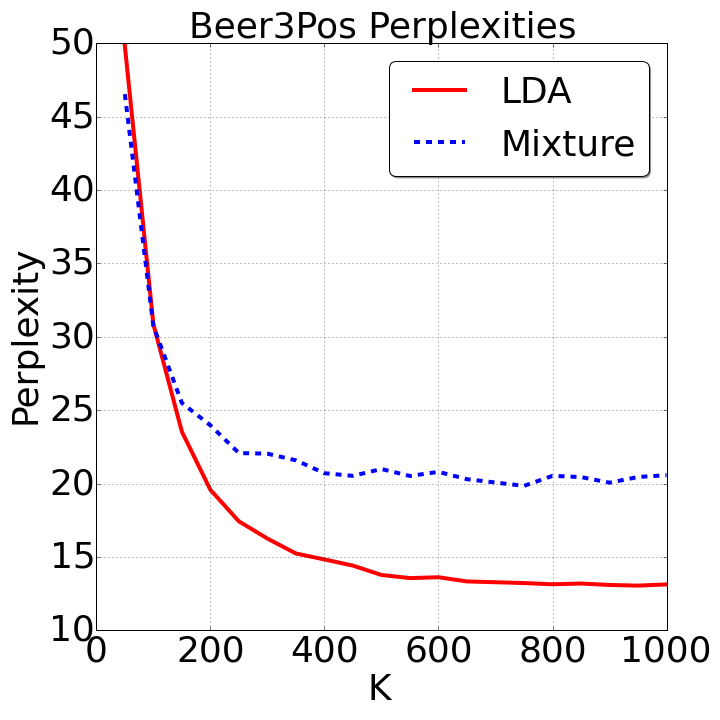
\includegraphics[width=0.5\linewidth]{07-lda/figures/perplexity.png}
\centering\caption{Results of model comparisons of LDA and multinomial mixture model on the Beer3 data. The lower perplexity values for $K>100$ demonstrates that LDA provides a better model fit on the held-out data when compared to the mixture model.\label{fig:m2lda-perplexity}}
\end{figure}

\subsection{Biochemical Analysis \label{sub:lda-biological-findings}}

With $K$ the number of Mass2Motifs set to 300 and other hyperparameters set to be the same as in cross-validation, Mass2Motifs were extracted for each Beer data and characterised by JvdH for biochemical relevance. As discussed in Section~\ref{sub:ms2lda-workflow}, the distributions over the features that make up the Mass2motifs and the distributions over Mass2motifs for each fragmentation spectrum can be thresholded in MS2LDAVis for results interpretation. For analysis, the threshold values of 0.05 and 0.01 for $t_{\theta}$ and $t_{\phi}$ were set, but they can easily be varied. The selection of these threshold values was based on JvdH's expert knowledge to allow for the extraction of a chemically-plausible set of features that comprise a Mass2Motif.

In the subsequent analysis that follows, Mass2Motifs with degrees ≥10 (i.e. that were present in ten or more spectra after thresholding) were manually inspected and annotated at different levels of confidence through integrating multiple supporting evidence such as the matching to a database of known reference standard compounds and spectral matching of the MS2 spectra containing the associated fragments and/or neutral losses to the reference spectra in MzCloud (www.mzcloud.org). Key fragment or loss features from the annotated Mass2Motifs in one sample were then searched against the list of Mass2Motifs in other samples and their correspondences established if those key fragment or loss features were present in both. 

Across the four Beer data, an average of 70\% of spectra (Table~\ref{tab:ms2lda-coverage}) include at least one annotated Mass2Motif, with Mass2Motifs related to the same substructure consistently found across multiple beers (e.g. hexose-related Mass2Motifs were present in all positive ionization mode files with degrees from 58 to more than 100), despite the fact that each sample was processed through the workflow independently. Between 30 to 40 Mass2Motifs in each of the Beer sample could be structurally annotated as corresponding to a diverse set of biochemical substructures, including amino acid related (i.e. histidine, leucine, tryptophan, and tyrosine), nucleotide related (i.e. adenine, cytosine, and xanthine), and other molecules such as cinnamic acid, ferulic acid, ribose and N-acetylputrescine. In general, the more Mass2Motifs present in a particular spectrum, the more specific our annotations can potentially become. An exhaustive identification effort to characterise all spectra (metabolites) present in the data was not attempted by JvdH, as it would be a major undertaking on its own, however it is noted that annotating just 30 to 40 of the discovered Mass2Motifs provide some structural biochemical insights into 70\% of the spectra. This suggests that a large percentage of metabolites can be automatically classified according to function (based on presence of functional groups or as a part of biological pathways). 

\begin{table}
\begin{centering}
\begin{tabular}{|c|c|c|c|}
\hline 
File & Total MS1 peaks & Linked to at least one structurally annotated M2M & \%\tabularnewline
\hline 
\hline 
Beer1Pos & 1282 & 951 & 74\tabularnewline
\hline 
Beer2Pos & 1567 & 1160 & 74\tabularnewline
\hline 
Beer3Pos & 1422 & 1055 & 74\tabularnewline
\hline 
Beer4Pos & 1363 & 930 & 68\tabularnewline
\hline 
\end{tabular}
\par\end{centering}
\caption{Mass2Motif coverage of MS1 peaks by percentage of MS1 peaks that can
be explained by at least one structurally annotated Mass2Motif for
the files acquired in positive ionization mode.\label{tab:ms2lda-coverage}}
\end{table}

As an example of the biochemical insights that can be obtained by an expert from MS2LDAVis, Figure~\ref{fig:m2lda-ferulic-acid} shows three of the eleven spectra that include Mass2Motif 19, characterised as corresponding to ferulic acid substructure. Ferulic acid is a compound found in the hard outer layer of grain (the bran) of cereals (an ingredient of beer) and is expected to be shared by the metabolites in beer as a substructure. Across the three spectra, we see conserved fragment and loss features shared by the spectra explained by Mass2Motif 19, with the most conserved features highlighted in Figure~\ref{fig:m2lda-ferulic-acid}D. Unlike MS2Analyzer \cite{ma2014ms2analyzer} where the prior information on the fragment features of interest has to be specified in advance, the discovery of conserved features in MS2LDA is performed in an unsupervised manner. In addition, JvdH verified that the \textit{loss_176.1086} feature in Figure~\ref{fig:m2lda-ferulic-acid}B is an informative feature related to the complete ferulic acid substructure. While this is easily observed from the visualisation, information on conserved patterns of neutral loss will be difficult to extract from any other tools apart from MS2LDA. The entire results in Figure~\ref{fig:m2lda-ferulic-acid} shows that through MS2LDA, we can extract a biochemically relevant pattern present in just eleven of the entire set ($>$1000) of spectra, although the individual spectra can be quite different. 

In a comparison to metabolite identification via spectral library matching using the NIST MS/MS database for small molecules (http://chemdata.nist.gov/mass-spc/msms-search/) and MassBank \cite{horai2010massbank}, only one from the eleven spectra explained by Mass2Motif 19 returns a ferulic acid related hit. This is despite the clear presence of fragment and loss features corresponding to ferulic acid substructure across the eleven spectra. Similarly, the beer metabolites explained by Mass2Motifs related to histidine, tyrosine, and tryptophan were subjected to spectral matching. In the verification by JvdH, matches to reference spectra were found for 33 spectra with 15 matches consistent with their characterised Mass2Motifs. These results demonstrate how MS2LDA effectively recognizes core substructures in mass spectral data and can serve as an aid to the classification and annotation of metabolites. Critically, it does this by matching only small portions of the spectra (substructures) rather than relying on complete spectral matches. In summary, for this subset of four Mass2Motifs, spectral matching allows classification of 45\% of the associated metabolites whereas MS2LDA is able to functionally annotate all of them. In addition, MS2LDA can annotate and group spectra based on neutral losses (e.g. the loss of a free carboxylic acid group) which is not possible via spectral matching.

\begin{figure}[!htbp]
\centering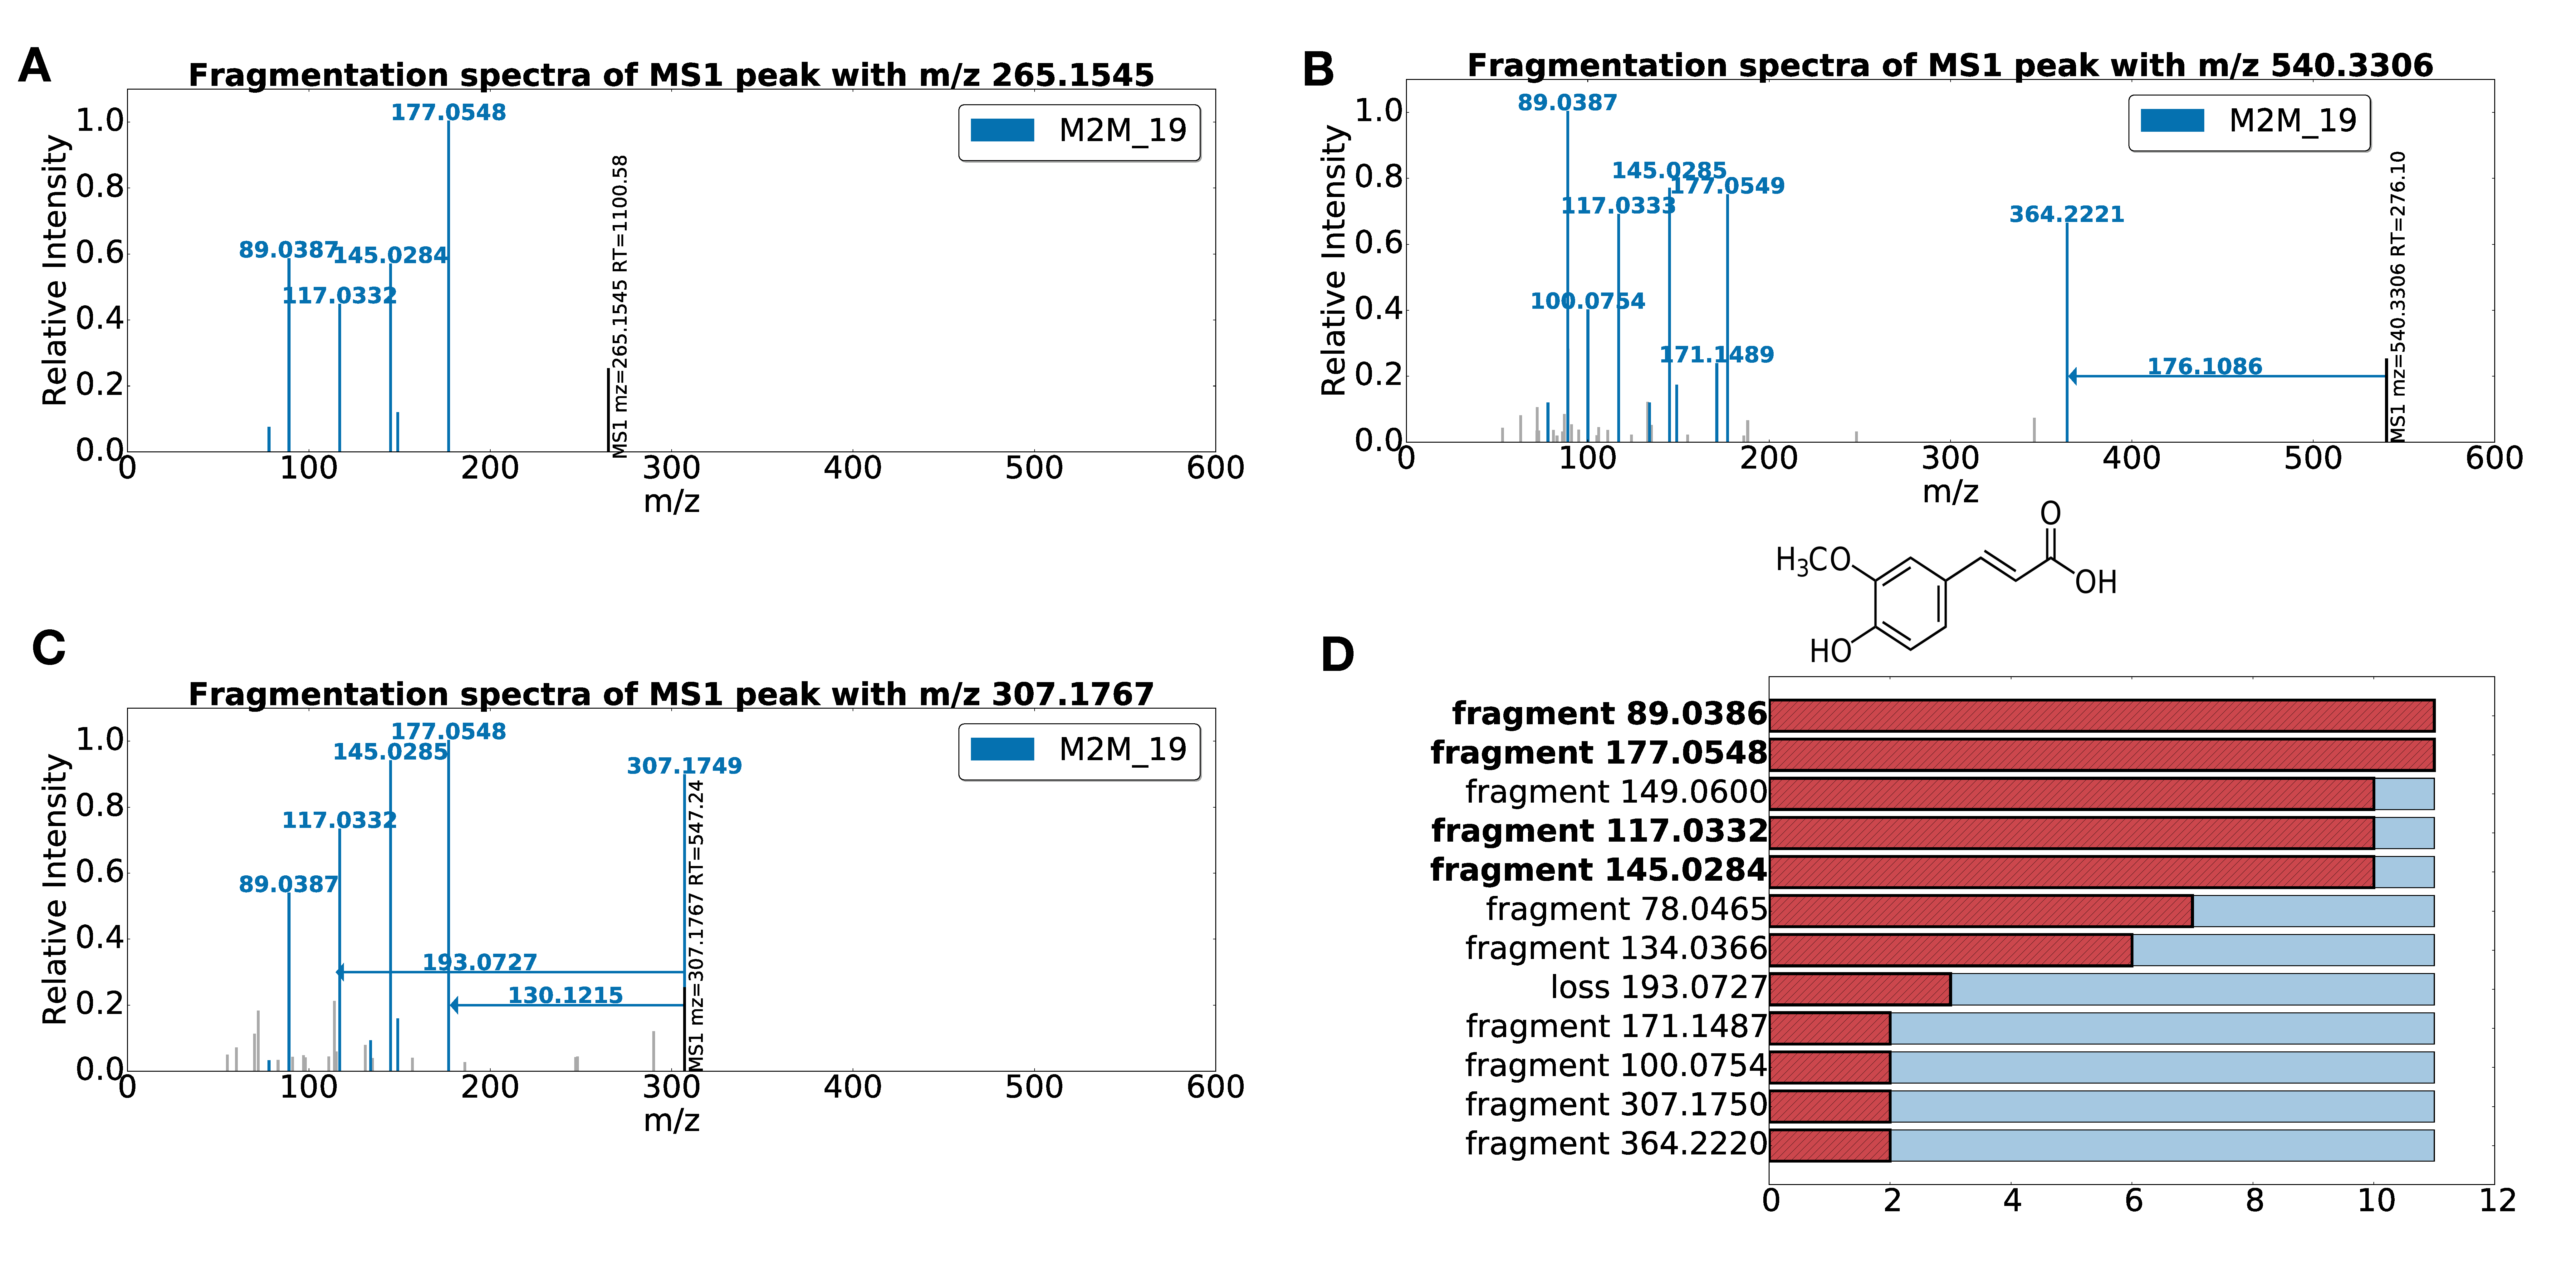
\includegraphics[width=0.8\linewidth]{07-lda/figures/figure3.pdf}
\centering\caption{Three spectra, from the beer3 positive ionization mode file, each of which includes Mass2Motif 19, annotated as the plant derived ferulic acid substructure. A-C highlight mass fragments and neutral losses (arrows originating at the precursor ions) included in Mass2Motif 19 (fragments not explained by Mass2Motif 19 are light grey). Ferulic acid substructure is illustrated at the top of D, while the boxplot in D shows how common each fragment or loss features (representative of the substructure) are found in the 11 spectra explained by Mass2Motif 19 found in the dataset. Features highlighted in bold are consistently present in Mass2Motifs inferred across the four beer samples.\label{fig:m2lda-ferulic-acid}}
\end{figure}

\subsubsection{Validation to Reference Standard Molecules}

Of the 45 molecules we were able to identify as standard molecules in one or more of the beer extracts, 38 can be explained by one or more annotated Mass2Motif, and 32 of the annotated Mass2Motifs correspond to known biochemical features that are consistent with the standard molecules. This demonstrates that characterised Mass2Motifs represent conserved patterns of metabolites' fragmentation spectra in authentic standard mixtures. Figure~\ref{fig:m2lda-standards} shows some examples for these fragmentation spectra coloured by characterised Mass2Motifs. The spectra for phenylalanine (Figure~\ref{fig:m2lda-standards}A) and histidine (Figure~\ref{fig:m2lda-standards}B) share Mass2Motif 262, and indeed feature \textit{loss\_46.0054}, which has been verified by JvdH as informative that a carboxylic acid group (CHOOH) is lost from the molecular ion during fragmentation, is a common characteristic of phenylalanine and histidine. Similarly, other Mass2Motifs (115, 241) in Figures~\ref{fig:m2lda-standards}A and~\ref{fig:m2lda-standards}B are related to phenylalanine and histidine compounds. Finally, Figure~\ref{fig:m2lda-standards}D is the MS2 spectrum of adenosine, which consists of an adenine molecule conjugated to a ribose sugar molecule. The two associated Mass2Motifs 156 and 220 correctly represent the two biochemically relevant substructures (i.e., adenine substructure and a loss corresponding to a ribose sugar). 

Note that in our analysis on these standard molecules, the inferred Mass2Motifs were characterised first without any prior knowledge on the identities of standard compounds, but we still observe a high level of agreements between the identifications of standard compounds and the independent characterisation of Mass2Motifs which explains identified spectra. This suggests an alternative to the usual procedure where identification is performed first and the common substructures, shared by the small set of identified compounds, are deduced. In the complementary approach, characterised Mass2Motifs can be used as a starting point for analysis. The large number of spectra that can be explained by Mass2Motifs are further examined and their putative identities deduced through collaborating multiple evidences, such as substructure annotation, matching against standard database, MS2 spectral library, etc. 

\begin{figure}[!htbp]
\centering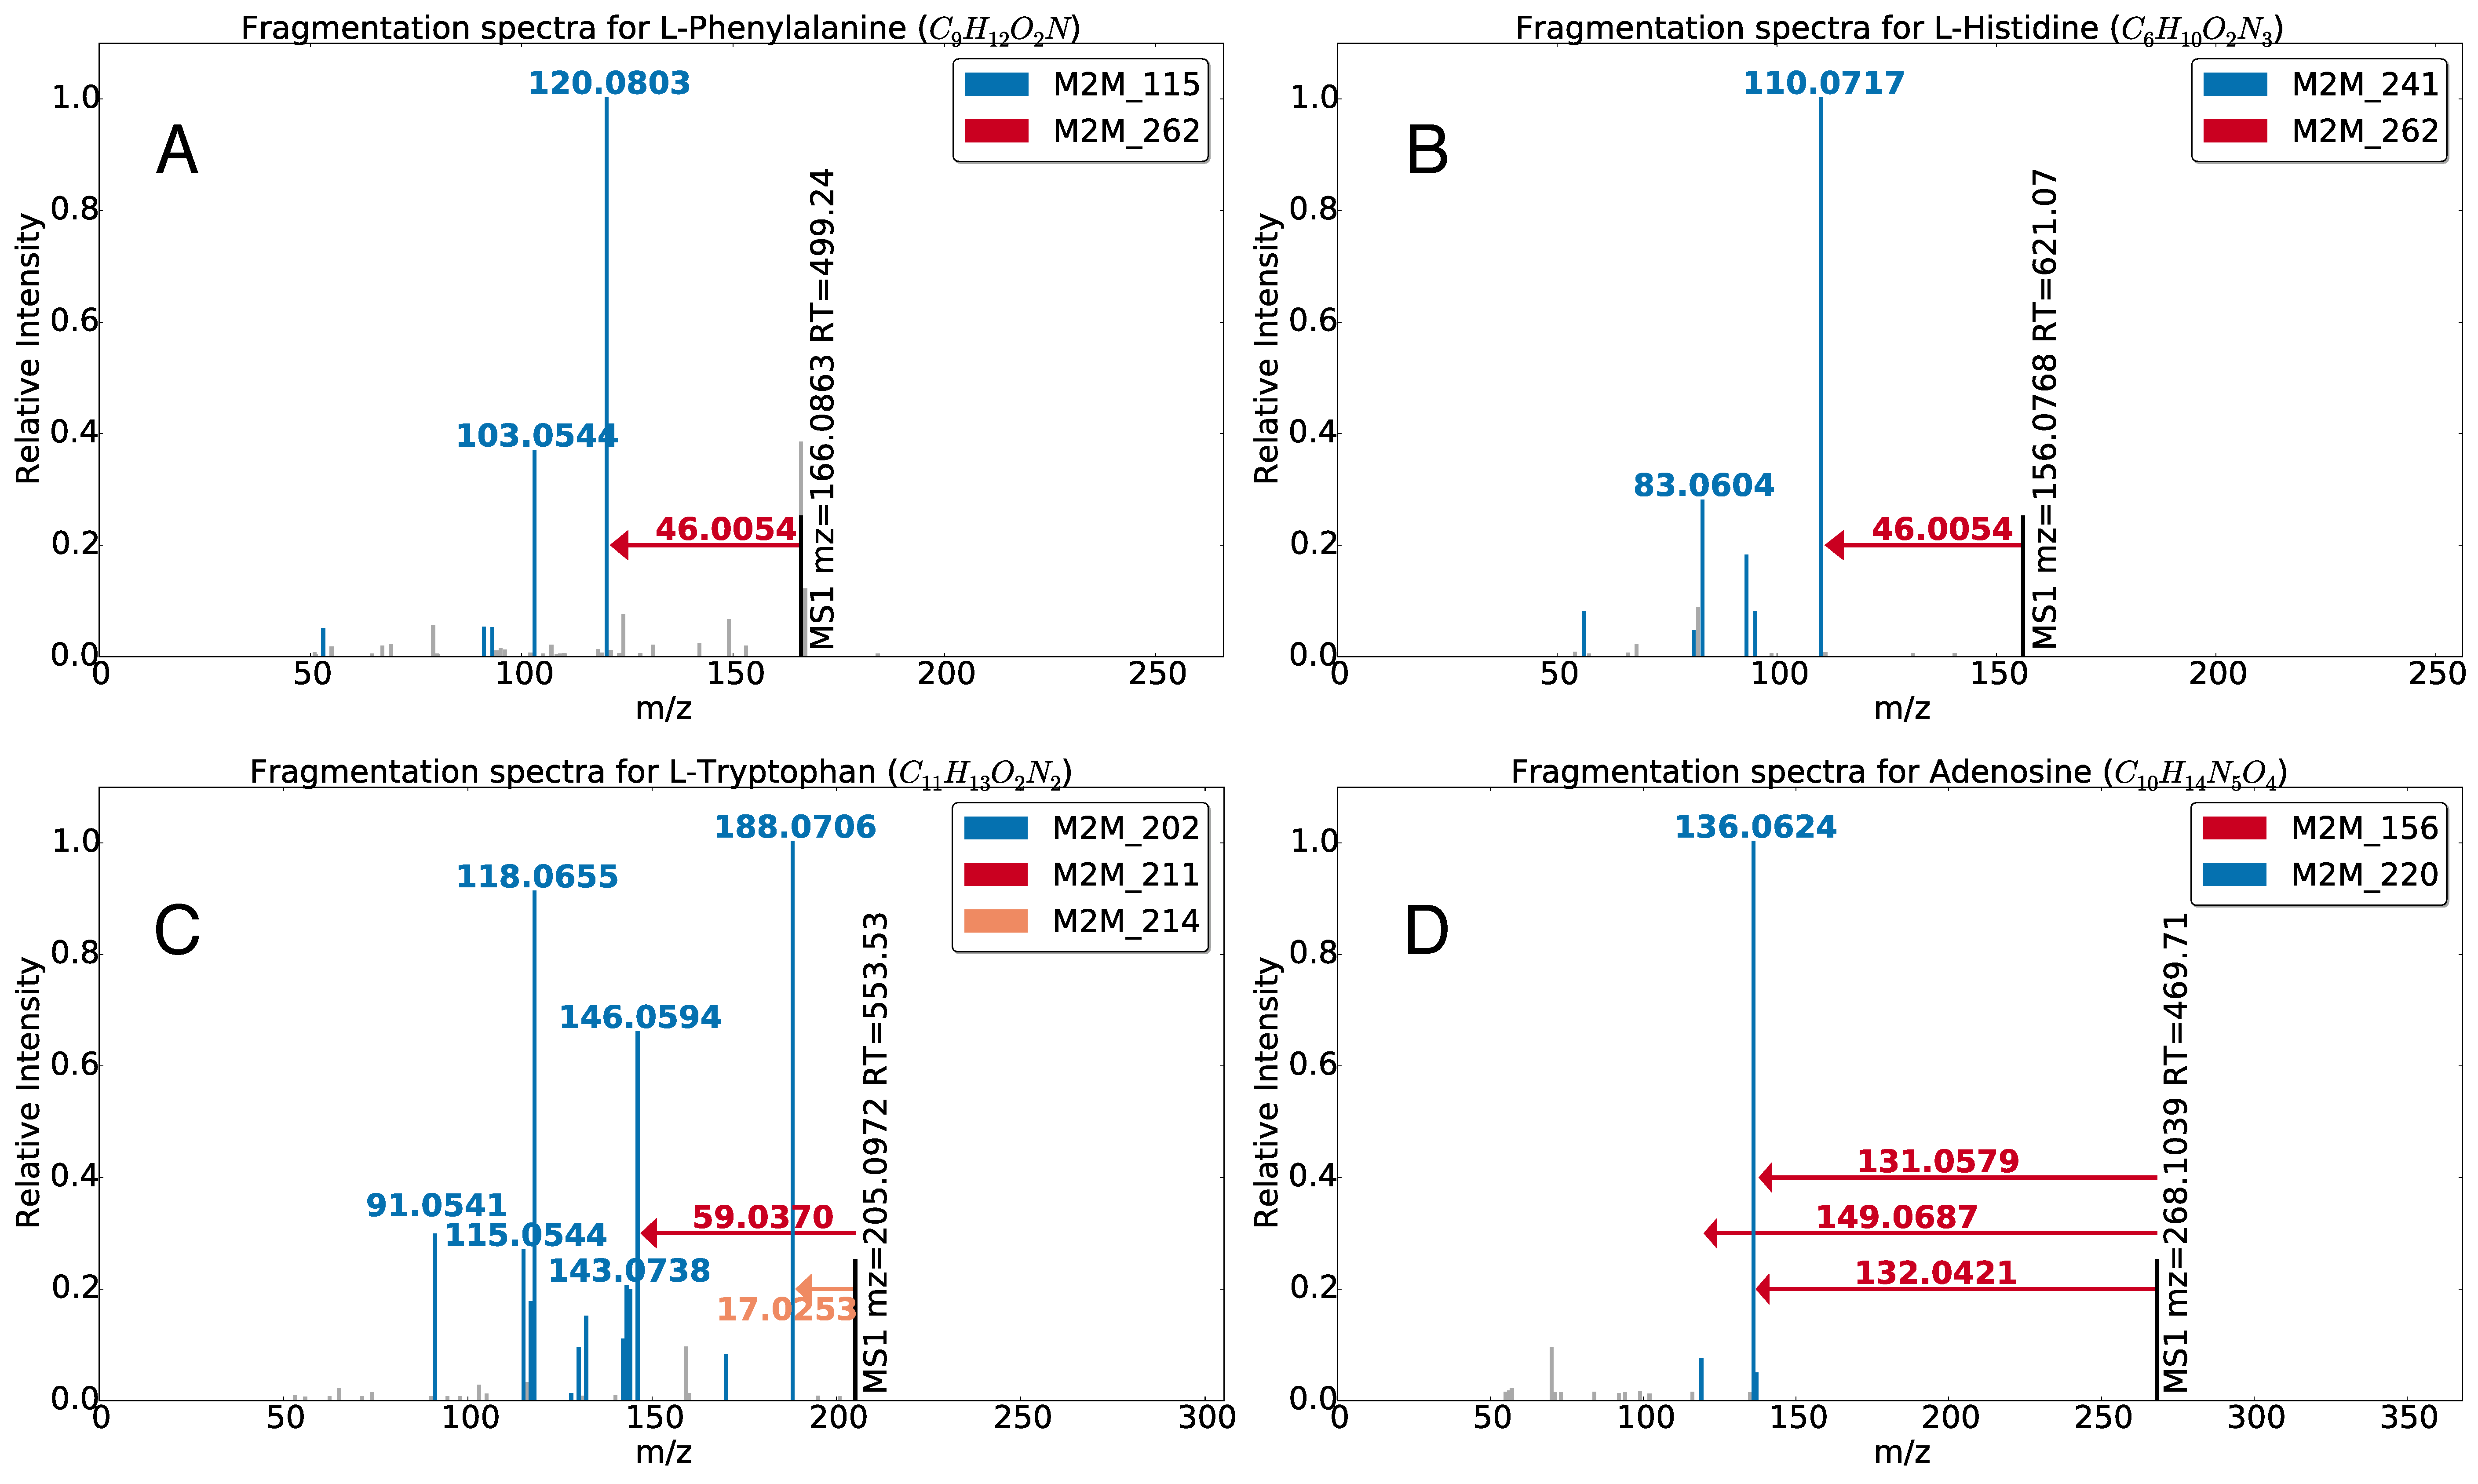
\includegraphics[width=0.8\linewidth]{07-lda/figures/standards.pdf}
\centering\caption{Mass2Motif spectra of identified standard molecules A) L-histidine, B) L-phenylalanine, C) L-tryptophan, and D) adenosine, with their characterized motifs (see Table~\ref{tab:ms2lda-standards}) indicated by colours.\label{fig:m2lda-standards}}
\end{figure}

% Preview source code for paragraph 1

\begin{table}
\small
\begin{centering}
\begin{tabular}{| c | p{4cm} | c | p{3.5cm} | p{2.5cm} |}
\hline 
Mass2Motif & Annotation & Degree & Fragment or Loss Features & Elemental Formula\tabularnewline
\hline 
\hline 
115 & {[}phenylalanine-CHOOH{]}-based substructure.  & 28 & fragment\_120.0808, fragment\_103.0546, fragment\_91.0541 & C8H10N, \newline C8H7, \newline C7H7\tabularnewline
\hline 
156 & {[}ribose (pentose, C5-sugar)-H2O{]}-related loss.  & 22 & loss\_132.0421 & C5H8O4 \tabularnewline
\hline 
202 & {[}tryptophan-NH3{]}-related substructure.  & 15 & fragment\_118.0654, 
fragment\_117.0571, 
fragment\_91.0541, 
fragment\_130.0645,
fragment\_188.0706 & C8H8N, \newline
C8H7N, \newline
C7H7, \newline
C9H8N, \newline
C11H10NO2\tabularnewline
\hline 
211 & N-acetylputrescine substructure.  & 24 & loss\_59.0370, \newline
fragment\_114.0912, 
fragment\_72.0447, 
fragment\_60.0448 & C2H5NO, 
C6H12NO, C3H6NO, 
C2H6NO\tabularnewline
\hline 
214 & amine loss.  & 57 & loss\_17.0247  & NH3\tabularnewline
\hline 
220 & adenine substructure.  & 32 & fragment\_136.0629, 
fragment\_119.0351 & C5H6N5, 
C5H3N4\tabularnewline
\hline 
241 & histidine substructure.  & 21 & fragment\_110.0718, 
fragment\_156.0769, 
fragment\_93.0450, 
fragment\_95.0608 & C5H8N3, 
C6H10N3O2, 
C5H5N2, 
C5H7N2\tabularnewline
\hline 
262 & combined loss of H2O and CO \textendash{} indicative for free carboxylic
acid group (COOH).  & 90 & loss\_46.0053  & CH2O2 \tabularnewline
\hline 
\end{tabular}
\par\end{centering}
\caption{Annotations of the Mass2Motifs associated to the fragmentation spectra
of the peaks generated by the standard molecules shown in Figure~\ref{fig:m2lda-standards}. The degree of
a Mass2Motif indicates the number of MS2 fragmentation spectra in
Beer3 positive ionization mode data having the fragment or loss features
that can be explained by the Mass2Motif. \label{tab:ms2lda-standards}}
\end{table}

\subsubsection{Comparison to Spectral Clustering}

Spectral clustering approaches (e.g. Molecular Networking) can also help in molecular annotation by propagating identifications through the network. For example, if one spectrum can be identified, it can be used to putatively annotate the spectrums neighbours in the network. MS2LDA differs from this approach in three key ways. Firstly, MS2LDA does not require any complete spectra to be identified (they can be putatively annotated from Mass2Motifs). Secondly, MS2LDA does not require a high degree of total spectral similarity to allow spectra to share annotations; it just relied on the presence of a shared Mass2Motif. Finally, because spectra can include multiple Mass2Motifs, they can be given multiple annotations while in spectral clustering, each spectrum can only belong to one cluster. A key characteristic of MS2LDAis the ability to decompose MS2 spectra into multiple (potentially biochemically relevant) components. For example, in each of Figures~\ref{fig:m2lda-standards}A to \ref{fig:m2lda-standards}D, we observe the spectra being decomposed into 2 or more Mass2Motifs. To our knowledge, no other methods can do this in an unsupervised manner without training spectra consisting of known structures or \textit{a priori} knowledge of interesting combinations of fragment and/or loss features.

Similarly in MS2LDA, a fragmentation spectrum can now be described by one or more Mass2Motifs. Figure~\ref{fig:m2lda-combined-m2m} demonstrates this with an example of a subset of the network produced by MS2LDAVis, consisting of spectra explained by two Mass2Motifs characterised as ferulic acid and ethylphenol. All but one spectrum can be explained by just one of the Mass2Motifs but one spectrum is generated by a molecule that contain both substructures and can therefore be explained by both Mass2Motifs. In the Molecular Networking analysis by JvdH, this spectrum is placed into the ethylphenol cluster, but its relationship with ferulic acid is lost. This results in a much less specific annotation of that spectrum. In contrast, the knowledge on the presence of both Mass2Motifs in the spectrum allows JvdH to assign it a putative compound identification of feruloyltyramine ([C18H20NO4]+) despite spectral matching producing no relevant hits. In general, the more Mass2Motifs present in a particular spectrum, the more specific our annotations can potentially become.

\begin{figure}[!htbp]
\centering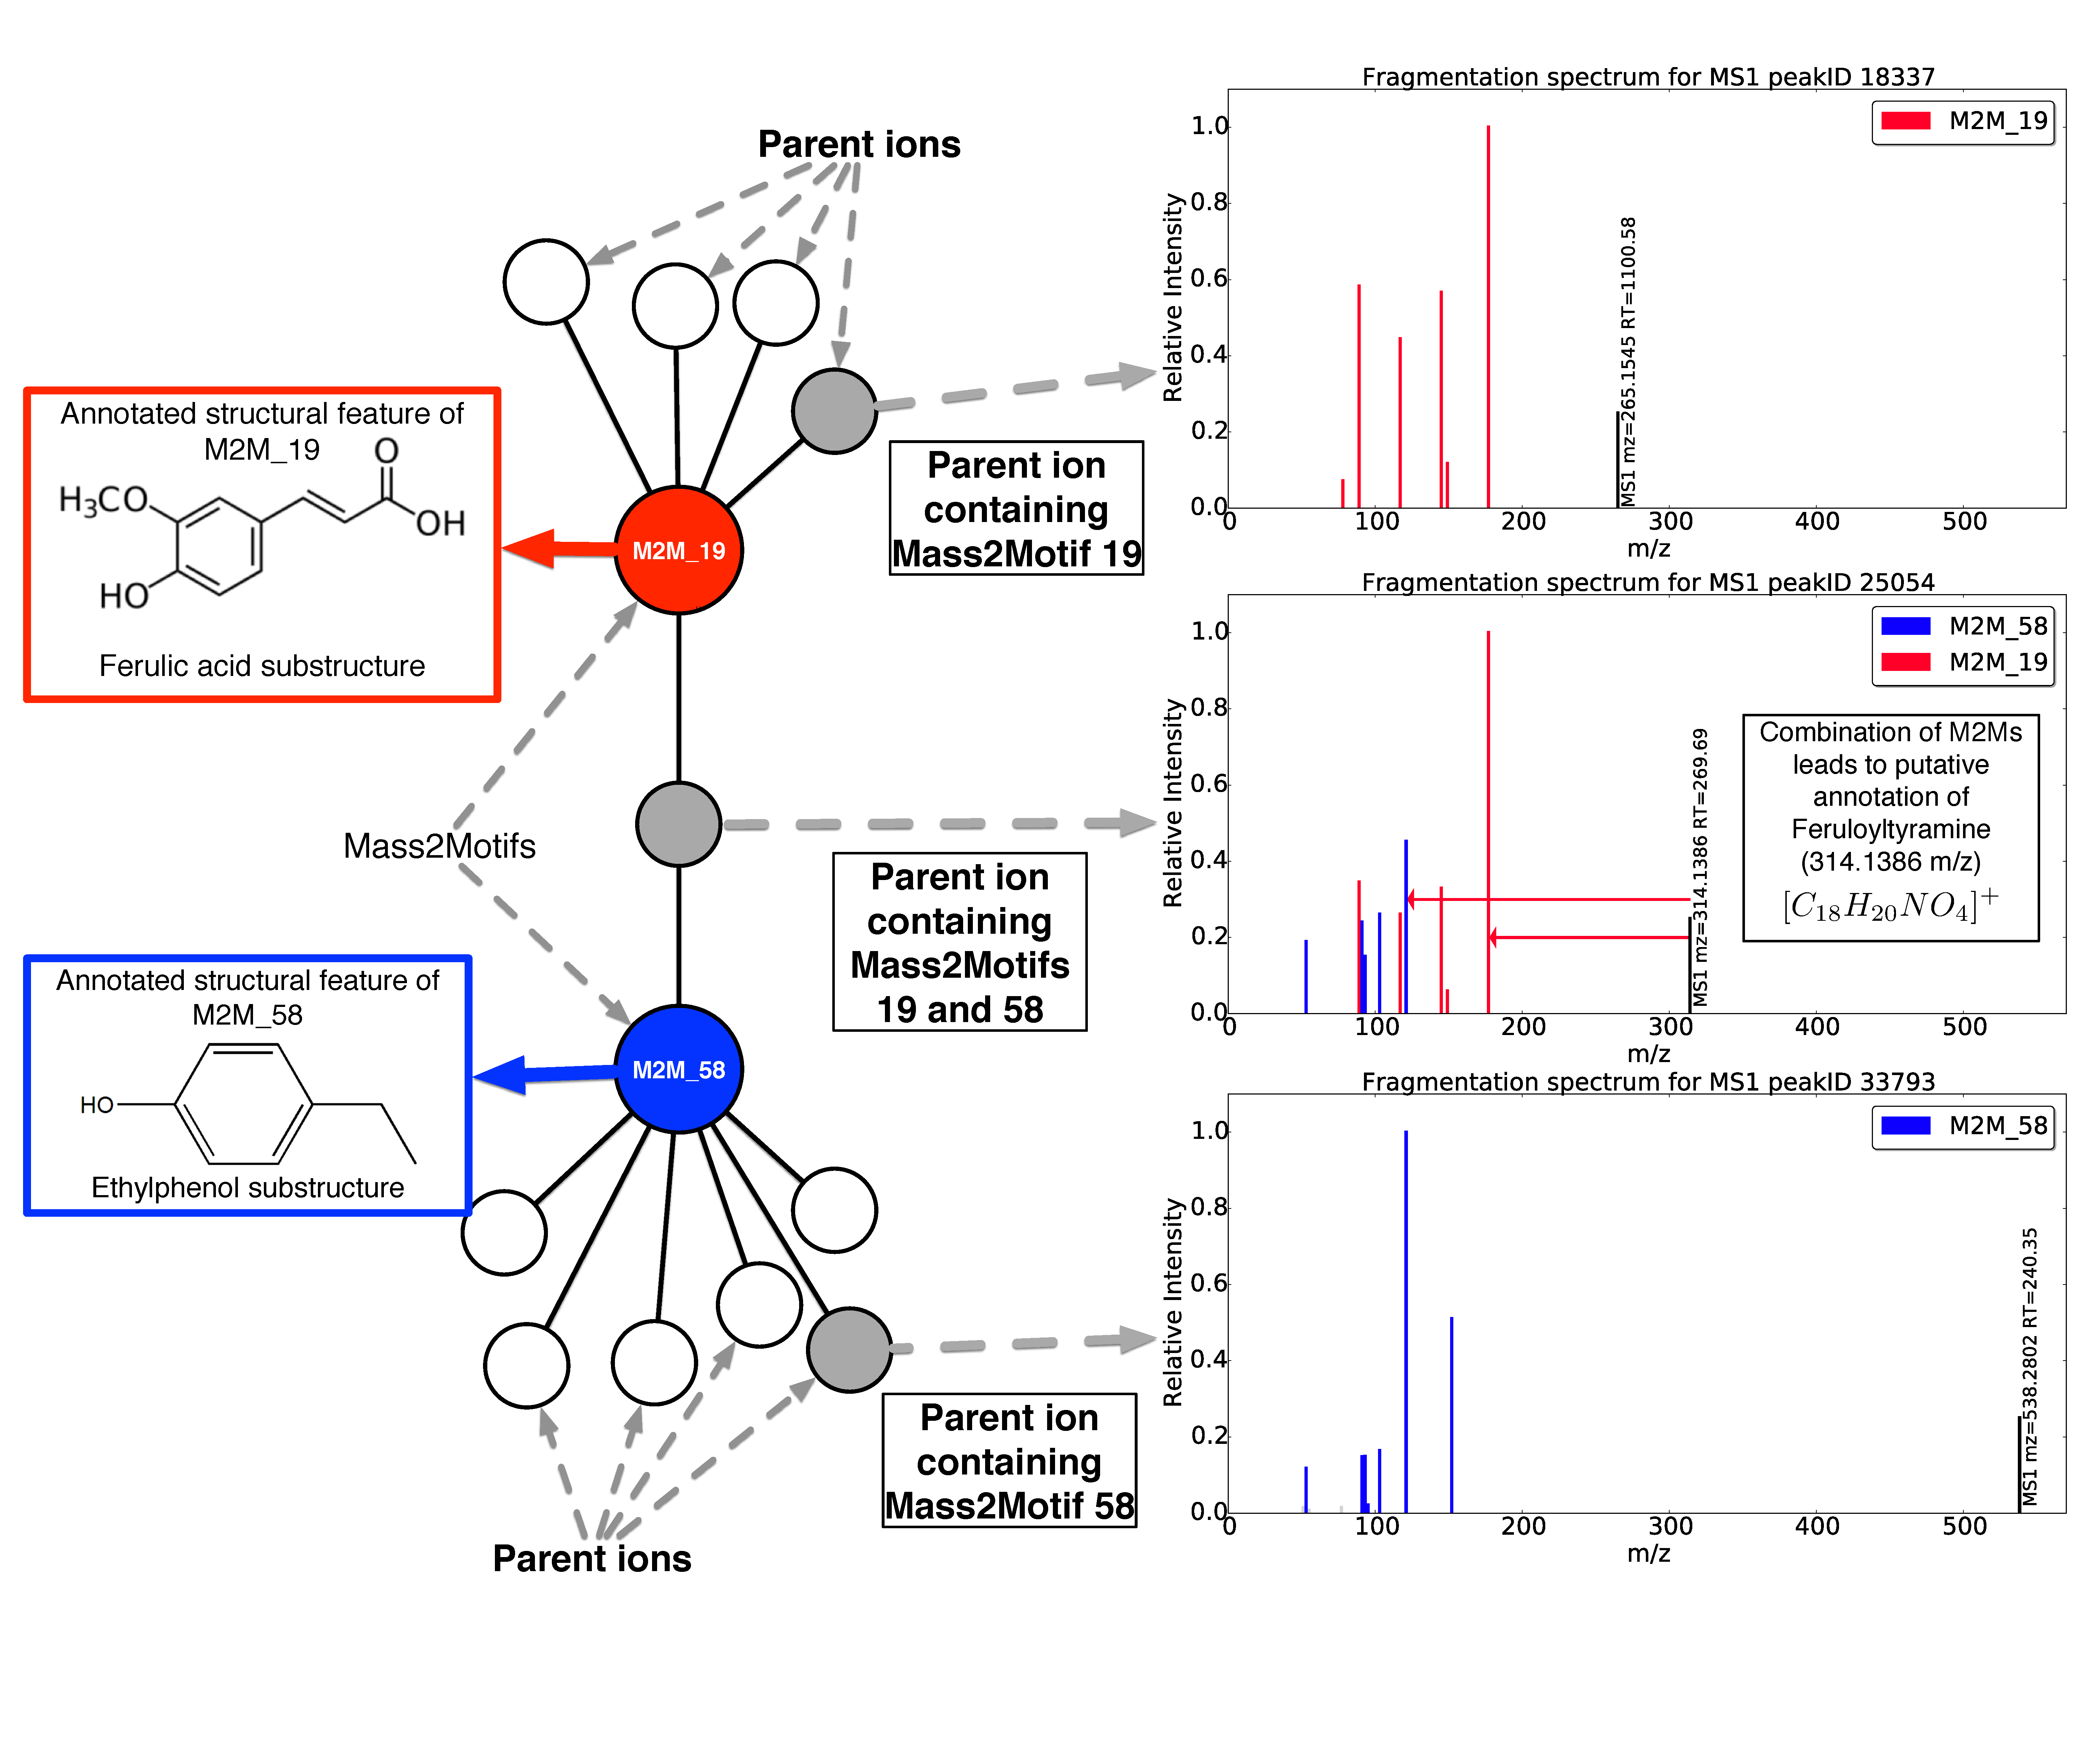
\includegraphics[width=1.0\linewidth]{07-lda/figures/combinedm2m.pdf}
\centering\caption{Mass2Motifs 19 and 58 were found to be representative of ferulic acid and ethylphenol, respectively. 11 fragmentation spectra can be explained by M2M_19, while 42 spectra can be explained by M2M_58. However, one spectra (shown as a gray node in the Figure) can be explained by both Mass2Motifs, but this is not possible in spectral clustering.\label{fig:m2lda-combined-m2m}}
\end{figure}

The same spectral clustering result is also reproduced in Figure~\ref{fig:m2lda-cosine-clustering} where a matrix of cosine similarities of the spectra, placed in the ferulic acid based cluster and the ethylphenol based cluster (from Molecular Networking). Two distinct groups of spectra, based on their cosine similarities, can be seen --- corresponding to each cluster. Members of each cluster can also be explained by a single Mass2Motif (the ferulic acid cluster by M2M_19, and the ethylphenol cluster by M2M 58). However, one spectrum (the last row in Figure~\ref{fig:m2lda-cosine-clustering}) can also be jointly explained by the two Mass2Motifs. In cosine clustering, this spectrum would have to go into one cluster or the other based on its cosine similarity and valuable information is lost. Since a compound consists of multiple substructures, allowing each spectra to be explained by multiple Mass2Motifs naturally results in a greater potential of producing a more comprehensive characterisations of the substructures of a compound. 

\begin{figure}[!htbp]
\centering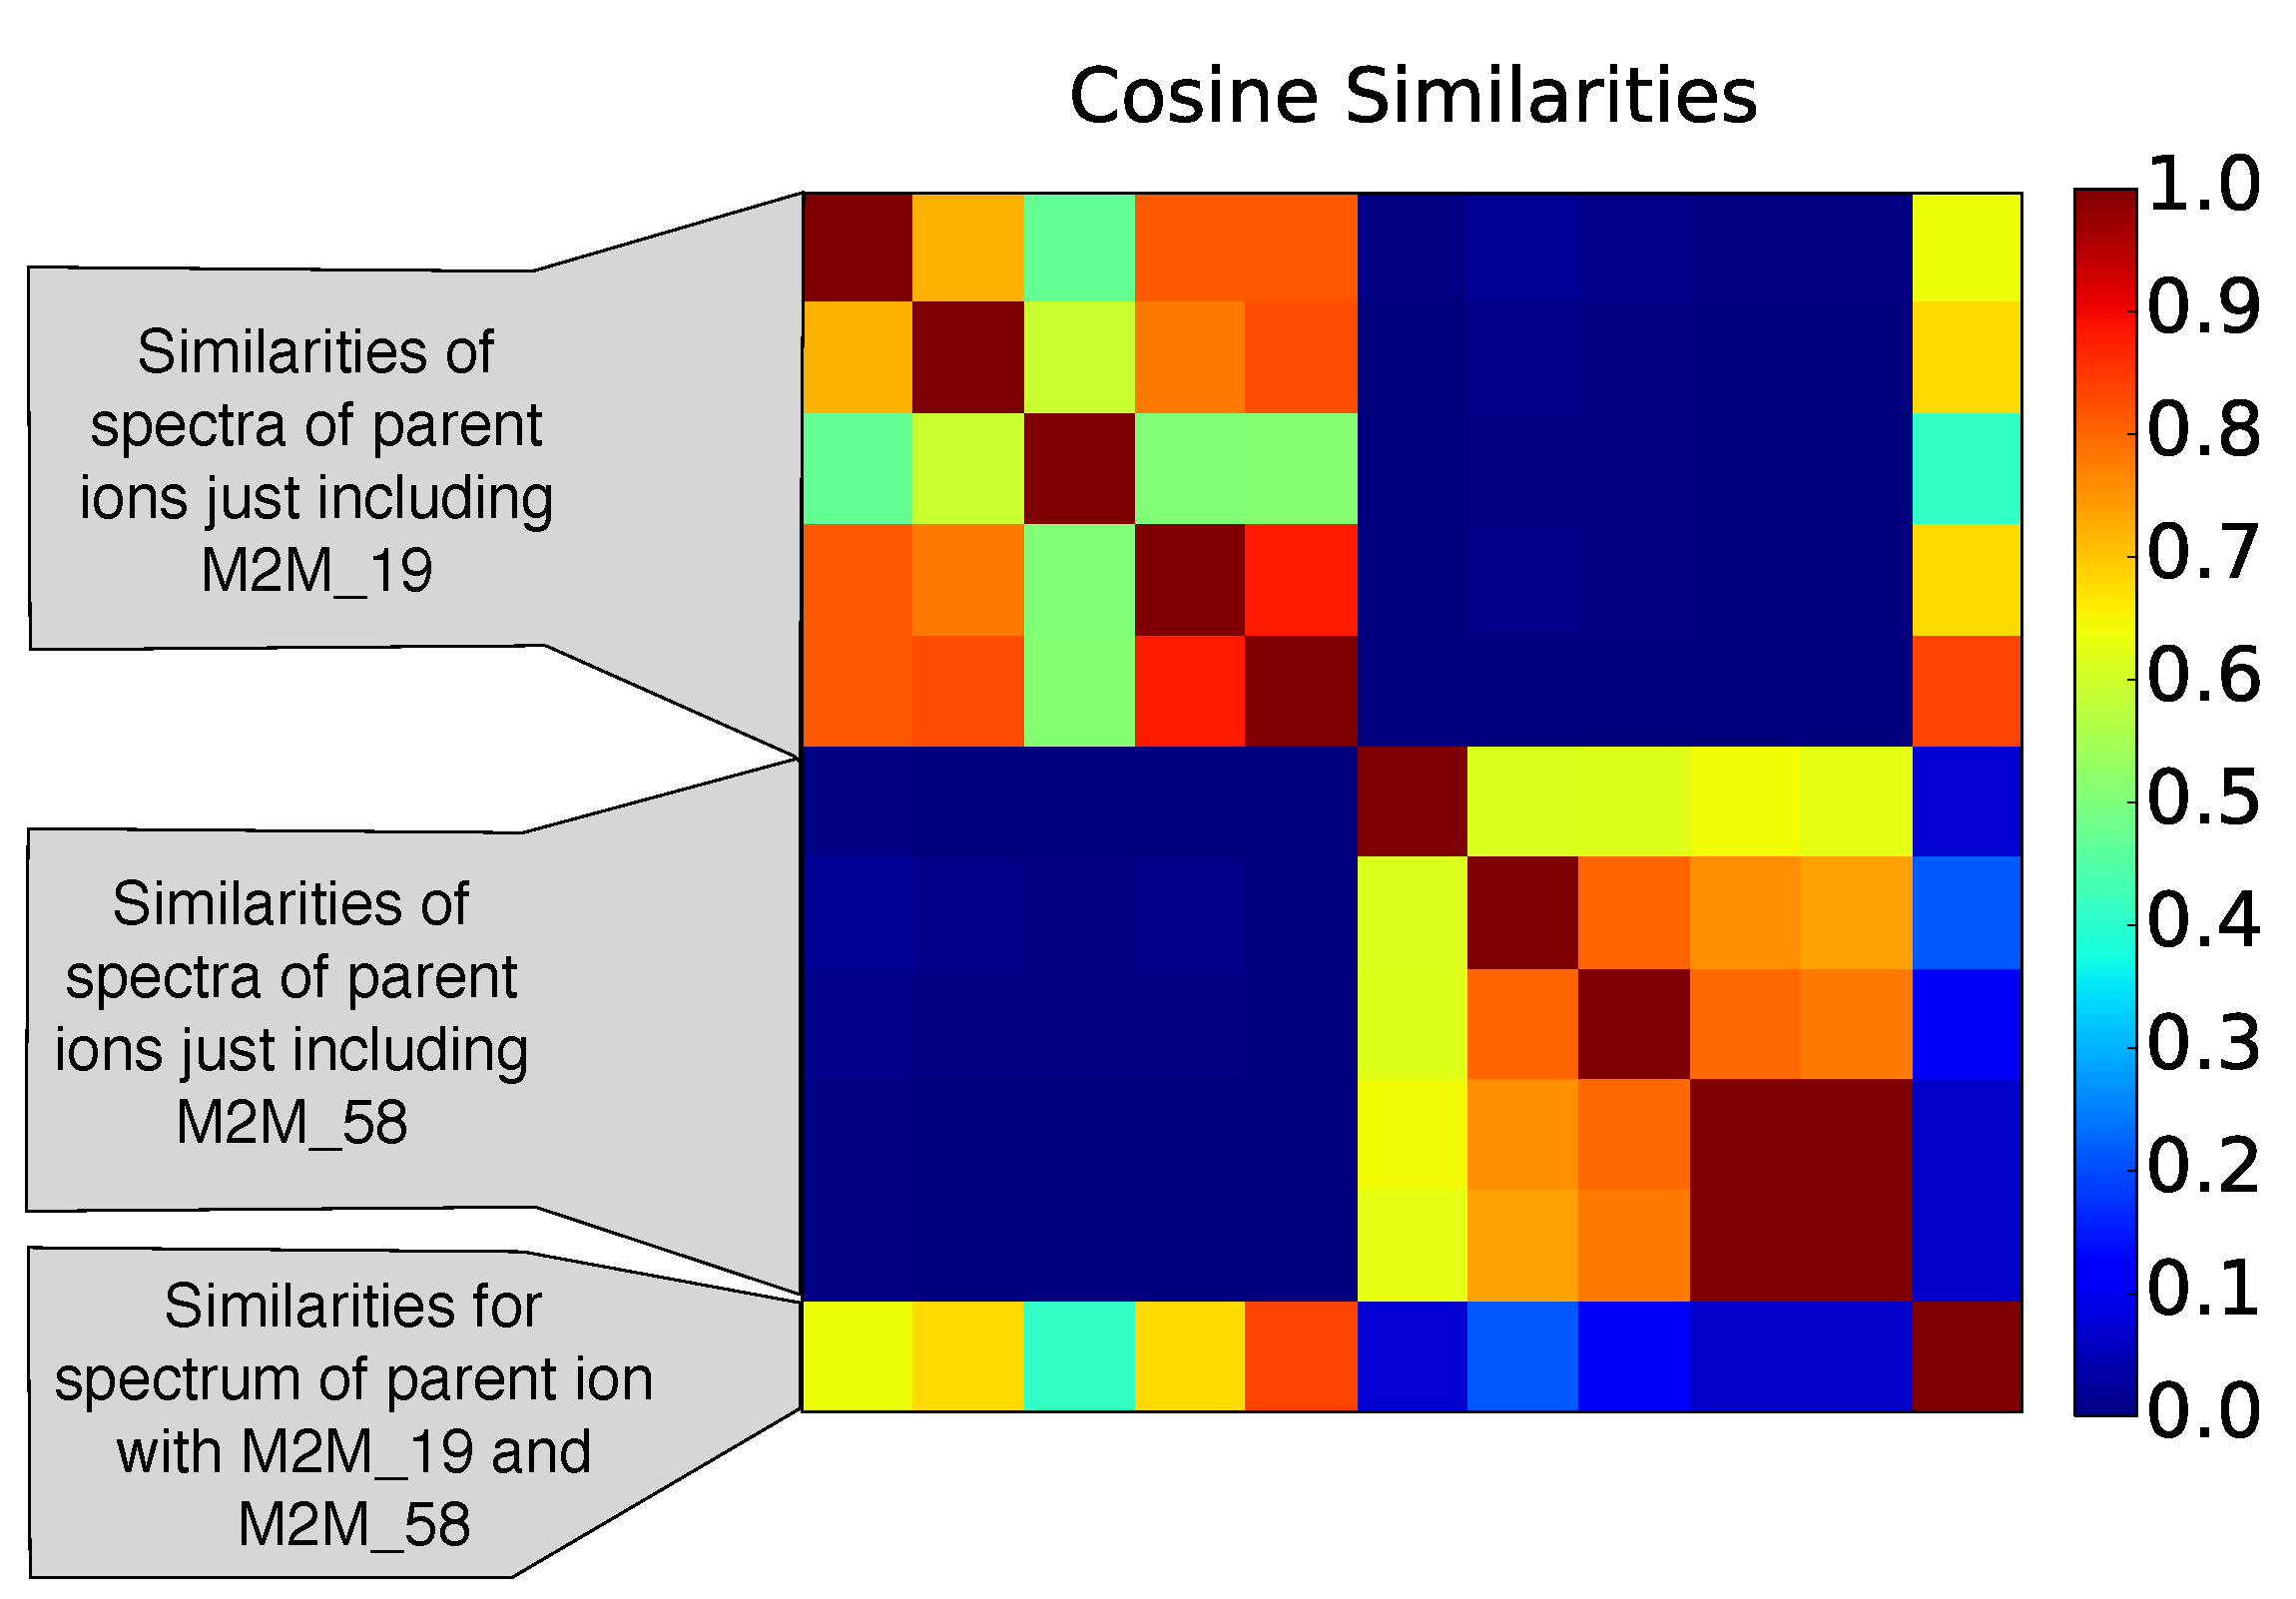
\includegraphics[width=0.6\linewidth]{07-lda/figures/figure10.pdf}
\centering\caption{Cosine clustering results of spectra drawn from the ferulic acid based cluster and the ethylphenol based cluster (similar to M2M_19 and M2M_58). The last row represents a fragmentation spectrum that contains both substructures, but in the clustering approach, the spectra will be placed into one of the clusters based on its cosine similarity. In LDA, this spectrum can be explained by Mass2Motifs that characterise both substructures.\label{fig:m2lda-cosine-clustering}}
\end{figure}

\subsubsection{Differential Analysis of Mass2Motifs}

We have shown that MS2LDA analysis can group molecules according to a shared Mass2Motif. As spectra can include multiple Mass2Motifs, so molecules can belong to multiple functional groups. In transcriptomic studies, it is common to consider the shared differential expression (DE) of a group of transcripts that are related through the sharing of the same Gene Ontology classification. The equivalent case in metabolomics are metabolites that share the same functional substructures and can potentially be mapped onto related pathways. The presence of the same functional substructure across these metabolites naturally suggest that their spectra can be described by the same Mass2Motif. If all metabolites sharing the same substructure are differentially expressed across samples, hypothesis can be generated as to the underlying biochemical significance causing the expression changes. From performing differential analyses on the expressions (intensity values) of metabolites having spectra explained by the same Mass2Motif, it is therefore possible to assess the biochemical changes of groups of metabolites across samples. Note that this does not depend on the small number of metabolites having spectra that can be identified through spectral matching, instead it relies on the much larger sets of MS1 peaks having spectra that can be jointly explained by a Mass2Motif.

Using PLAGE \cite{tomfohr2005pathway}, we assessed the DE of each Mass2Motif based on the intensity changes of the relevant MS1 peaks between beers 2 and 3. Figure~\ref{fig:m2lda-heatmaps} shows MS1 intensities of metabolites explained by two Mass2Motifs (characterised as guanine and pentose loss) with high PLAGE scores. In each case, the change in intensity across the two beer extracts are very clear (note that PLAGE considers changes in both directions when scoring). Within the molecules having spectra explained by the guanine Mass2Motif, we could annotate 5-guanine containing metabolites and identify 2 to through matching to reference standards (Figure~\ref{fig:m2lda-heatmaps}A). For the pentose Mass2Motif, we could annotate 8 and identify 5 pentose-containing metabolites from the Mass2Motif (Figure~\ref{fig:m2lda-heatmaps}B). These biochemically relevant metabolites show interesting patterns in the DE between the two beers. As an example of how MS2LDA differential analysis can support hypothesis generation for an expert, JvdH noted that in Beer3, the free guanine is present more often, whereas in Beer2, the conjugates of guanine are more abundant (Figure~\ref{fig:m2lda-heatmaps}A). This reflects the differences in the chemical components of the two beers. Similarly, as metabolites can include multiple Mass2Motifs, JvdH observed that the four spectra (in Figures~\ref{fig:m2lda-heatmaps}) annotated as guanine-related metabolites (i.e., guanosine, two methyl-guanosine isomers, and a pentosyl-hexosylguanine) are also connected to the pentose loss Mass2Motif, which itself was also differentially expressed between the two beers. Indeed, the structures of those metabolites all share both a guanine and a pentose substructure. A comparison made by JvdH to Molecular Networking results revealed that in the standard spectral similarity approach, these spectra were distributed over 10 spectral clusters. In other words, the interesting structural and intensity similarity between these molecules exposed by MS2LDA would not be found via spectral clustering. 

% Figure~\ref{fig:m2lda-heatmaps} shows MS1 intensities of metabolites explained by two Mass2Motifs with high PLAGE scores (note that for a high PLAGE score changes in expression do not need to be in the same direction). As an example of the kind of biochemical insight this provides, in Beer3, the free guanine (Figure~\ref{fig:m2lda-heatmaps}A) is more abundant whereas in Beer2, guanine-conjugates are more abundant. Similarly, the molecules associated to the pentose Mass2Motif (Figure~\ref{fig:m2lda-heatmaps}B) show DE between the extracts. It is the grouping performed by MS2LDA that exposes such insights from fragmentation data. We investigated whether or not similar outcomes can be achieved with with spectral similarity clustering. With this approach, the 12 pentose-related metabolites were distributed across 10 clusters rather than appearing in a single grouping, hiding the potentially relevant correlated intensity change. Comparing against spectral similarity clustering, the molecules explainable by the pentose Mass2Motif (Figure~\ref{fig:m2lda-heatmaps}B) are distributed over 10 spectral clusters. The results suggest how MS2LDA analysis can be used to pull together the sets of fragment and loss features for differential analysis that would otherwise have not been found through spectral similarity clustering alone.

\begin{figure}[!htbp]
\centering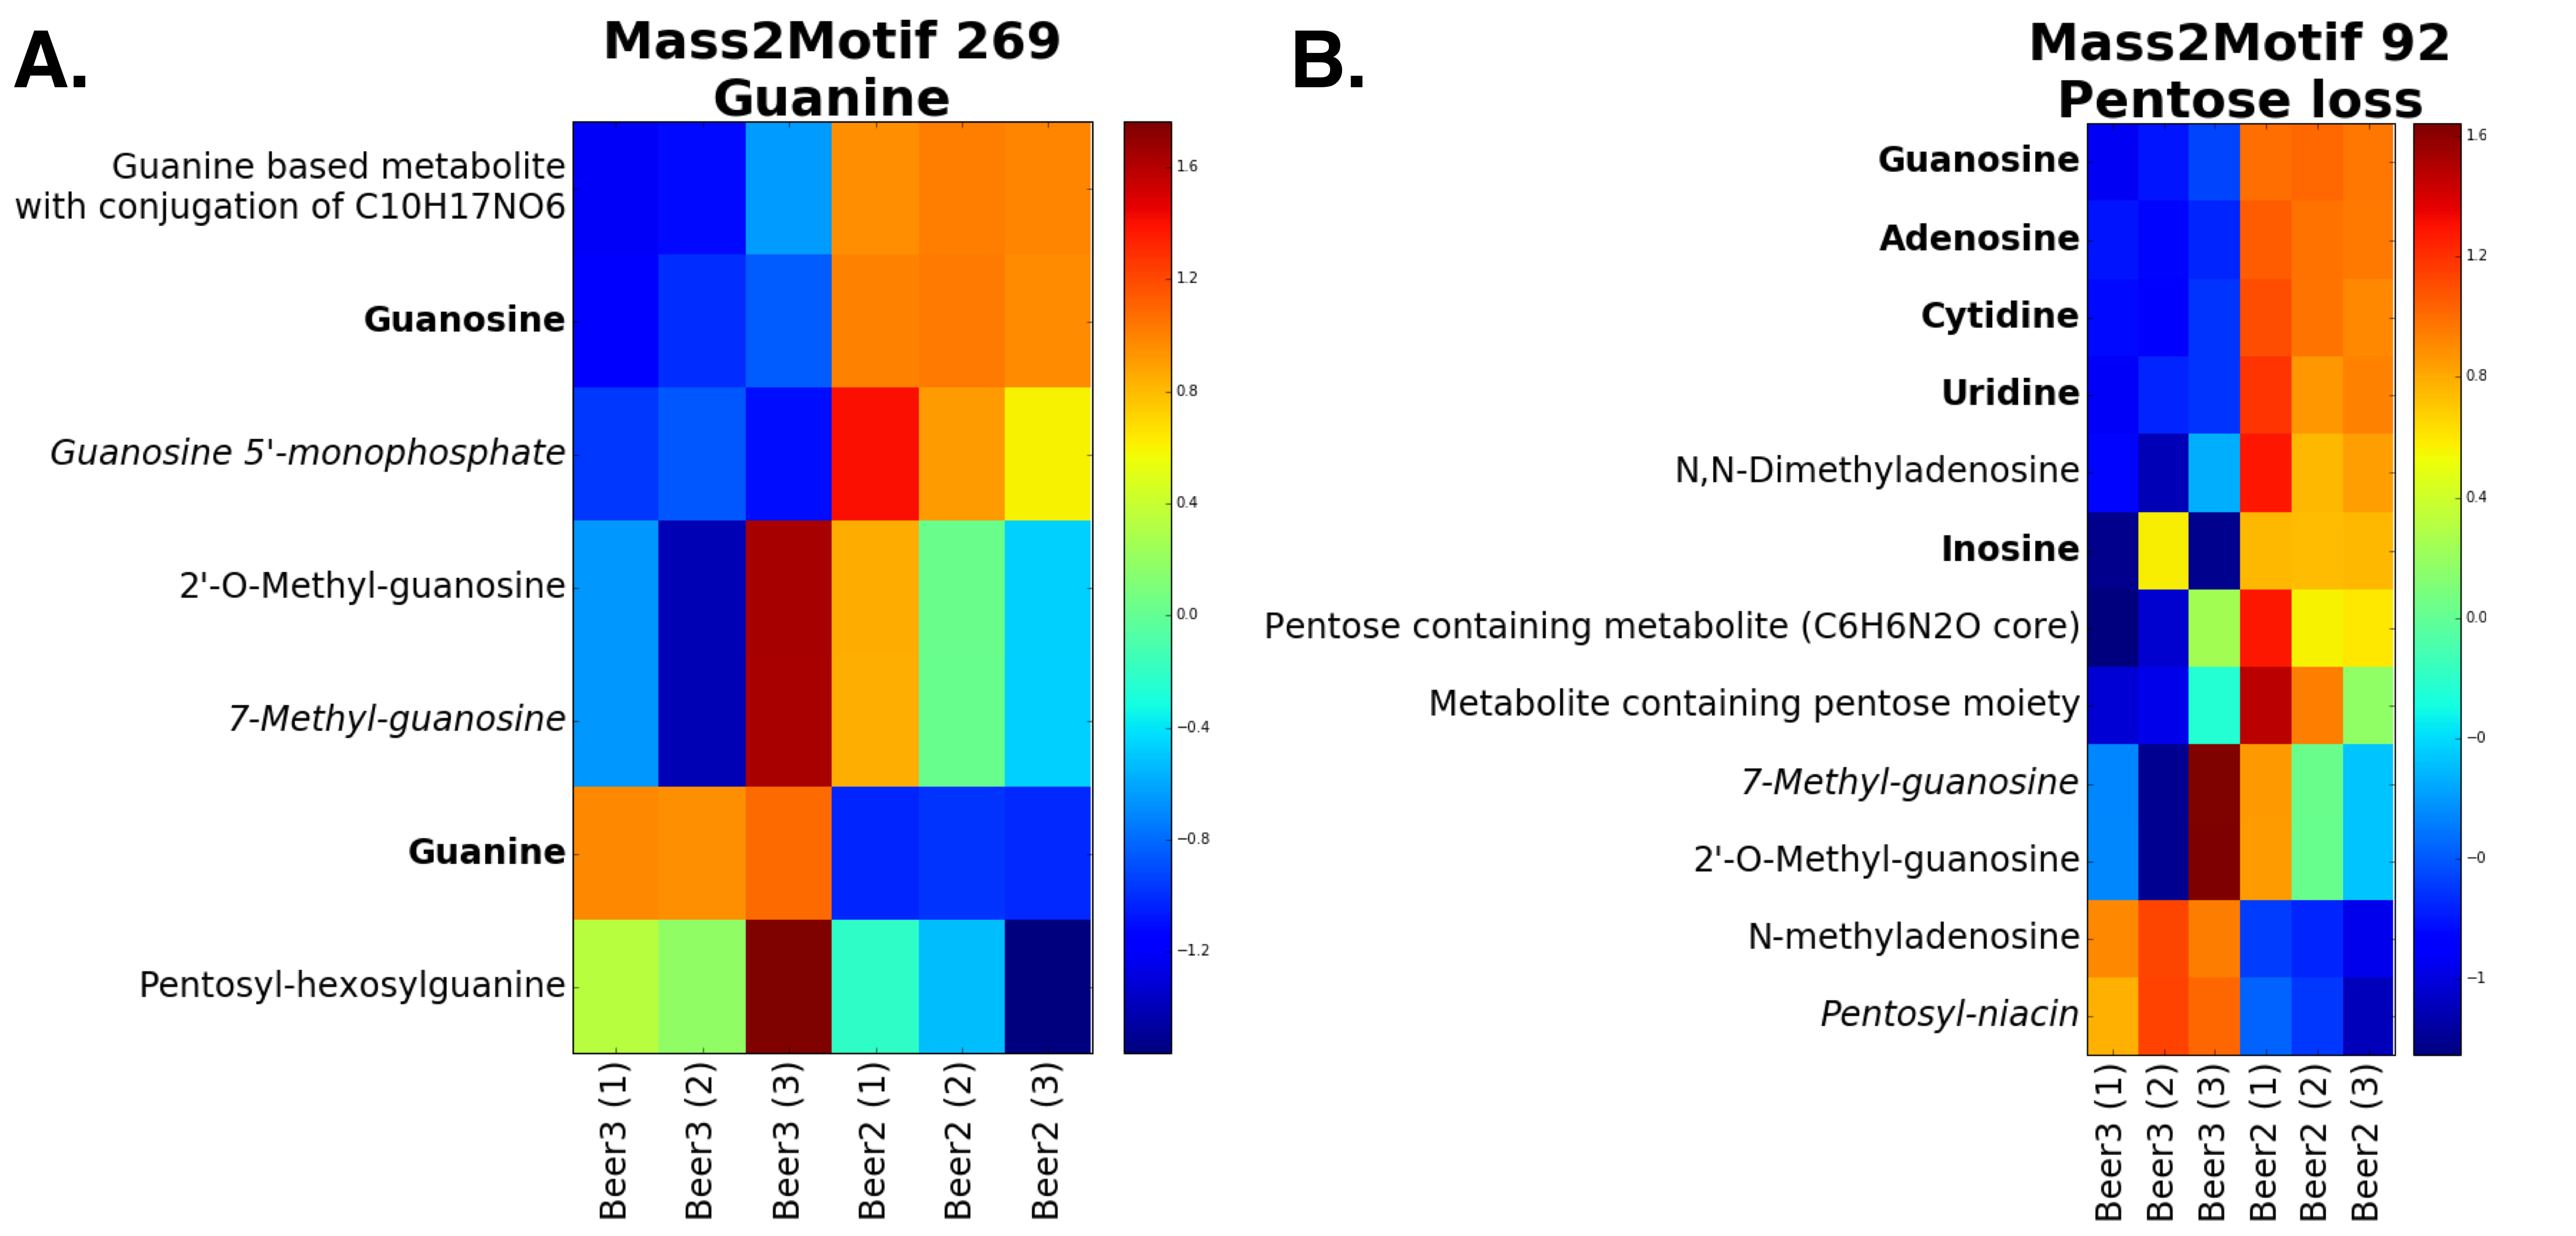
\includegraphics[width=1.0\linewidth]{07-lda/figures/heatmaps.png}
\centering\caption{Log fold change heat-maps for the A) guanine and B) pentose loss Mass2Motifs. Each row is an annotated parent MS1 peak and columns represent different beer extracts. Bold names for parent MS1 peaks could confidently be matched to reference compounds, while italic names are for those that are annotated at a lower degree of confidence. \label{fig:m2lda-heatmaps}}
\end{figure}

\section{Substructure Discoveries Across Many Fragmentation Files}

Manual inspection of the results revealed that many Mass2Motifs, related to the same substructures, are consistently present in two or more beers. This is despite each sample being processed independently through MS2LDA. For example, the hexose-related Mass2Motifs are present in all positive ionization mode beer files with degrees from 58 to more than 100 in each beer. The results suggest that we can jointly model the presence or absence of Mass2Motifs across many input files at once, eliminating the necessary but tedious matching of Mass2Motifs across files if they were to be inferred independently for each input file.

\subsection{Multi-file LDA Model}

Metabolomics dataset consist of fragmentation spectra in multiple input files, where each file is generated from measurements of a technical or biological replicate. In this manner, Mass2Motif distributions over fragment and loss features are shared across files, but within each file, fragmentation spectra have their own file-specific probabilities of observing certain Mass2Motifs. When only a single input file is provided, the multi-file LDA model reduces to the standard LDA model. 

In the proposed multi-file LDA model, the observation on the $n$-th fragment or loss feature in the $d$-th fragmentation spectra in file $f$ ($w_{dn}^f$) is conditioned on the assignment of feature $w_{dn}^f$ to some $k$-th global Mass2Motif multinomial distribution that is shared across files. This assignment is denoted by the indicator variable $\boldsymbol{z}_{dn}^f$, so $\boldsymbol{z}_{dn}^f=k$ if feature $n$ from fragmentation spectra $d$ in file $f$ is assigned to the $k$-th Mass2Motif. The probability of seeing certain Mass2Motifs for each $d$-th fragmentation spectra in file $f$ is then drawn from a multinomial distribution with a parameter vector $\boldsymbol{\theta}_{d}^f$. This parameter vector $\boldsymbol{\theta}_{d}^f$ is in turn drawn from a prior Dirichlet distribution having the parameter vector $\boldsymbol{\alpha}^f$. 
\begin{align}
\boldsymbol{z}_{dn}^f \vert \boldsymbol{\theta}_{d}^f &\sim Multinomial(\boldsymbol{\theta}_{d}^f) \label{eq:dir-multi-1a}\\
\boldsymbol{\theta}_{d}^f \vert \boldsymbol{\alpha}^f &\sim Dirichlet(\boldsymbol{\alpha}^f) \label{eq:dir-multi-1b}
\end{align}
As in the case of standard LDA, the $k$-th multinomial distribution for a Mass2Motif is characterised by the parameter vector $\boldsymbol{\phi}_{\boldsymbol{z}_{dn}^f}$, with $\boldsymbol{\phi}_{\boldsymbol{z}_{dn}^f}$ drawn from a prior Dirichlet distribution having the parameter vector $\boldsymbol{\beta}$. 
\begin{align}
\boldsymbol{w}_{dn}^f \vert \boldsymbol{\phi}_{\boldsymbol{z}_{dn}^f} &\sim Multinomial(\boldsymbol{\phi}_{\boldsymbol{z}_{dn}^f}) \label{eq:dir-multi-2a} \\
\boldsymbol{\phi}_{k} \vert \boldsymbol{\beta} &\sim Dirichlet(\boldsymbol{\beta}) \label{eq:dir-multi-2b}
\end{align}

Inference in the multi-file LDA model is again performed via a collapsed Gibbs sampling scheme. The conditional probability of $P(\boldsymbol{z}_{dn}^f=k \vert \boldsymbol{w}_{dn}^f, ...)$ of the assignment of feature $n$ in spectra $d$ file $f$ to Mass2Motif $k$ is given by eq. (\ref{eq:multifile-lda-gibbs}).
\begin{equation}
P(\boldsymbol{z}_{dn}^f=k \vert \boldsymbol{w}_{dn}^f, ...) \propto P(\boldsymbol{w}_{dn}^f \vert \boldsymbol{z}_{dn}^f=k, ...) P(\boldsymbol{z}_{dn}^f=k \vert ...)
\label{eq:multifile-lda-gibbs}
\end{equation}
where $...$ denotes any other parameters being conditioned upon but not explicitly listed. Similar to the derivation of standard LDA, we can marginalise over all $\boldsymbol{\phi}_k$ parameters in the likelihood term, $P(\boldsymbol{w}_{dn}^f \vert \boldsymbol{z}_{dn}^f=k, ...)$ of eq. (\ref{eq:multifile-lda-gibbs}), to obtain:
\begin{equation}
P(\boldsymbol{w}_{dn}^f \vert \boldsymbol{z}_{dn}^f=k, ...) \propto \frac{\sum_{f} c_{kn}^f + \boldsymbol{\beta}_n}{\sum_{n}\sum_{f} c_{kn}^f + \boldsymbol{\beta}_n}
\label{eq:multifile-lda-gibbs-likelihood}
\end{equation}
where $\sum_{f} c_{kn}^f$ is the total number of the $n$-th feature from all files currently assigned to Mass2Motif $k$ (this count excludes the current feature being sampled in the current iteration of Gibbs sampler). For the prior term $P(\boldsymbol{z}_{dn}^f=k \vert ...)$, marginalising over all $\boldsymbol{\theta}_{d}^f$ parameters produces as in the standard LDA:
\begin{equation}
P(\boldsymbol{z}_{dn}^f=k \vert ...) \propto  c_{dk}^f + \boldsymbol{\alpha}^f_k
\label{eq:multifile-lda-gibbs-prior}
\end{equation}
with $c_{dk}^f$ the number of features from document $n$ in file $f$ currently assigned to Mass2Motif $k$, excluding the current feature being sampled. 
Putting the prior and likelihood terms together, the following predictive distribution is obtained for the assignment of feature $n$ from document $d$ file $f$ to Mass2Motif $k$:
\begin{equation}
P(\boldsymbol{z}_{dn}^f=k \vert \boldsymbol{w}_{dn}^f, ...) \propto (c_{dk}^f + \boldsymbol{\alpha}^f_k) \cdot \frac{\sum_{f} c_{kn}^f + \boldsymbol{\beta}_n}{\sum_{n}\sum_{f} c_{kn}^f + \boldsymbol{\beta}_n}
\label{eq:multifile-lda-gibbs-combined}
\end{equation}

In each iteration of the Gibbs sampling, the information on the current feature $n$ in spectra $d$ file $f$ being sampled is removed. Reassignment of the feature to a Mass2Motif is then performed by sampling $\boldsymbol{z}_{dn}^f$ from the distribution specified by eq. (\ref{eq:multifile-lda-gibbs-combined}). Given $\boldsymbol{z}$, the predictive distribution for the $d$-th spectrum over the Mass2Motifs, $\boldsymbol{\theta}_{d}^f$, is obtained from the expectation of the Dirichlet-Multinomial distribution defined in eqs. (\ref{eq:dir-multi-1a})-(\ref{eq:dir-multi-1b}):
\begin{align}
\boldsymbol{\hat{\theta}}_{dk}^f = \frac{c_{dk}^f+\boldsymbol{\alpha}^f_k}{\sum_{k} c_{dk}^f+\boldsymbol{\alpha}^f_k}
\end{align}
where $c_{dk}^f$ is the count of features from spectra $d$ in file $f$ assigned to Mass2Motif $k$. 

For each spectra, the multinomial count vector $\textbf{c}_d^f$, of features from the spectra that are assigned to the different Mass2Motifs, is a sample from the Dirichlet-Multinomial distribution defined in eqs. (\ref{eq:dir-multi-1a})-(\ref{eq:dir-multi-1b}). Given all the $\textbf{c}_1^f,\textbf{c}_2^f, ... \textbf{c}_D^f$ vectors in the file, the parameter $\boldsymbol{\alpha}^f$ of the Dirichlet-Multinomial distribution of spectra-to-Mass2Motifs in file $f$ can be estimated by maximizing the log likelihood $log\prod_{d=1}^{D}  p(\boldsymbol{c}_{d}^f \vert \boldsymbol{\alpha}^f)$. An iterative procedure to approximate this is described in \cite{Minka2003}. The lower bound on the log likelihood of the multinomial data given $\boldsymbol{\alpha}^f$ is obtained from the iterative update:
\begin{equation}
\boldsymbol{\alpha}^f_k=\boldsymbol{\alpha}^f_k \frac{\sum_{d} \Psi(c_{dk}^f + \boldsymbol{\alpha}_k^f)-\Psi(\boldsymbol{\alpha}_k^f)}{\Psi(c_{d}^f + \sum_{k} \boldsymbol{\alpha}_k^f)-\Psi(\sum_{k} \boldsymbol{\alpha}_k^f)}
\end{equation}
where $\Psi(x)=\frac{\Gamma^{'}(x)}{\Gamma(x)}$ is the digamma function.

In a similar manner, for each $k$-th Mass2Motif, the predictive distribution over features, $\boldsymbol{\phi}_k$, can be obtained as the expectation of the Dirichlet-Multinomial distribution defined in eqs. (\ref{eq:dir-multi-2a})-(\ref{eq:dir-multi-2b}):
\begin{align}
\boldsymbol{\hat{\phi}}_{kn} = \frac{c_{kn}+\boldsymbol{\beta}_n}{\sum_{n} c_{kn}+\boldsymbol{\beta}_n}
\end{align}
where $c_{kn}$ is the count of the $n$-feature from all files that are assigned to Mass2Motif $k$. 

\subsection{Results \& Discussion}

On the dataset of four Beer extracts in positive ionisation mode processed through multi-file LDA using the same hyperparameters as the individual LDA. For data interpretation, initially, the same threshold values on $t_{\theta}$ and $t_{\phi}$ were selected as the previous single-file analysis (0.05 and 0.01 respectively). Table~\ref{tab:multifile-results} shows the results of five global Mass2Motifs that could be matched to the individual LDA results in Section~\ref{sub:lda-biological-findings}. The results in Table~\ref{tab:multifile-results} shows that multi-file LDA produces comparable results on the Mass2Motifs composition. This is entirely expected given that the four Beer extracts used for evaluation share similar metabolic profiles and correspondingly, have many substructures in common. 

\begin{table}[!tbhp]
\small
\centering
\begin{tabular}{|l|l|p{3.8cm}|}
\hline
Mass2Motif & Annotation                & Top Features Above Threshold                                                                                                                                                                           \\ \hline
M2M\_17           & Ferulic acid substructure & \textbf{fragment\_177.05478}, \textbf{fragment\_89.03865}, \textbf{fragment\_145.02844}, \textbf{fragment\_117.03319}, loss\_58.98941, \newline fragment\_163.03887, \textbf{fragment\_149.05998}, loss\_88.09967 \\ \hline
M2M\_155          & Histidine substructure    & \textbf{fragment\_110.07161}, \textbf{fragment\_156.07687}, fragment\_83.06041, \textbf{fragment\_93.04511}, fragment\_82.05246, fragment\_209.10558, \textbf{fragment\_95.06057}, loss\_167.08663, fragment\_81.04494, loss\_191.0615 \\ \hline
M2M\_115          & Leucine substructure      & \textbf{fragment\_86.09653}, \textbf{fragment\_132.10165}, fragment\_69.07013, fragment\_332.112, fragment\_143.11763 \\ \hline
M2M\_95           & Water loss substructure   & \textbf{loss\_18.01031}, \newline fragment\_314.0859, \newline fragment\_296.07259                                                                                                              \\ \hline
M2M\_232          & Asparagine substructure   & \textbf{fragment\_136.06231}, loss\_162.03459, \textbf{fragment\_119.0354}, loss\_162.00534, \newline fragment\_137.04623 \\ \hline
\end{tabular}
\caption{Five global Mass2Motifs inferred from multi-file LDA. For each Mass2Motif, the top features above threshold are listed. Features characterised as key to the substructure from the previous individual LDA analyses are shown in bold.}
\label{tab:multifile-results}
\end{table}

Information from all files now contribute to the inference of global Mass2Motifs. The fact that global Mass2Motifs that are consistent with our previous characterisation in Section~\ref{sub:lda-biological-findings} still emerge suggests the same underlying patterns of fragment and loss features to be present in each Beer extract. Figure~\ref{fig:multifile-lda} shows four example fragmentation spectra originating from different Beer extracts --- jointly inferred by multi-file LDA as containing the Mass2Motif characterised as the ferulic acid substructure. While this can be achieved from independently running LDA on each file, the tedious matching process of common Mass2Motifs across files can now be eliminated. Inspections on the degree (the number of spectra associated to a Mass2Motif above the user-defined threshold $t_{\theta}$) of the five Mass2Motifs in Table~\ref{tab:multifile-results} revealed that with a minor adjustment to $t_{\theta}$, the same sets of fragmentation spectra previously associated to the listed Mass2Motifs can all be recovered. 

\begin{figure}[!htbp]
\centering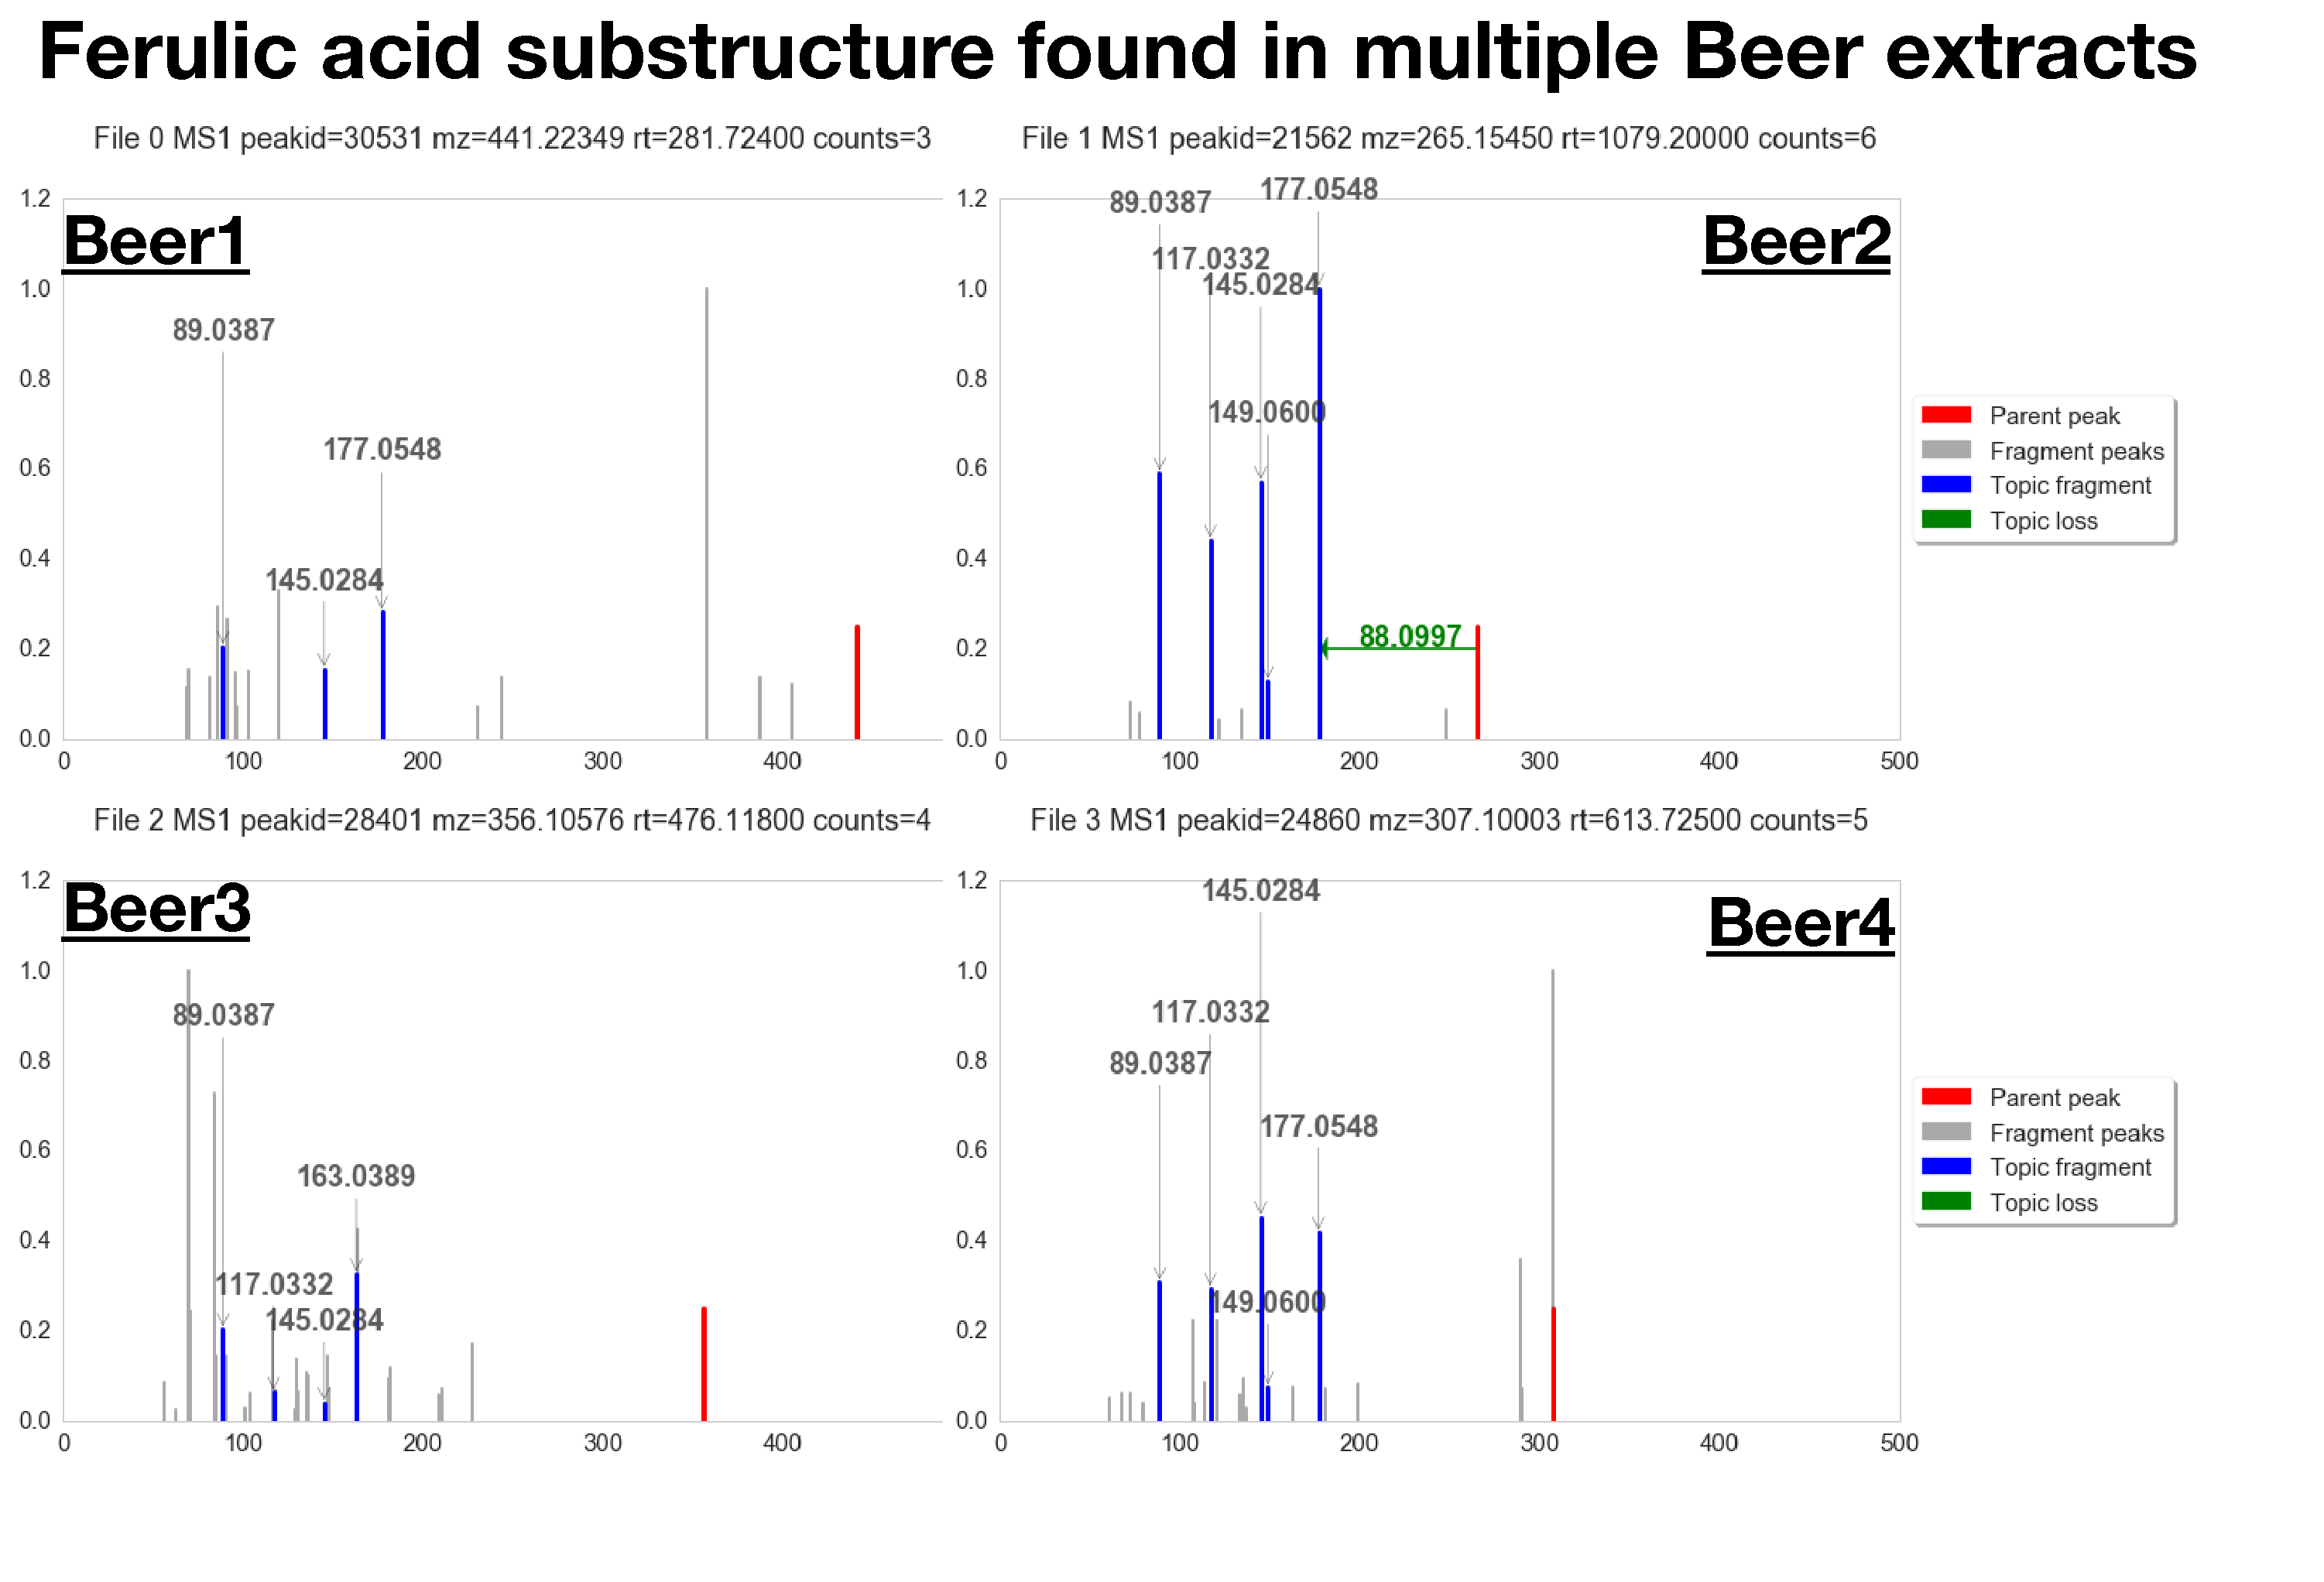
\includegraphics[width=1.0\linewidth]{07-lda/figures/multifile.pdf}
\centering\caption{Fragmentation spectra from different Beer extracts found by multi-file LDA to contain the same Mass2Motif (M2M_17) characterised as the ferulic acid substructure.\label{fig:multifile-lda}}
\end{figure}

From each posterior sample, we can also obtain the updated $\boldsymbol{\alpha}^f$ for the different Mass2Motif across all files. As $\boldsymbol{\alpha}^f$ is the asymmetric parameter that serves as the pseudo-count in the Dirichlet-Multinomial distribution of spectra-to-Mass2Motifs, a high value of $\boldsymbol{\alpha}^f_k$ for a particular $k$ means that a specific Mass2Motif is more likely for each spectra in file $f$. Figure~\ref{fig:multifile-lda-alpha} shows the plot of posterior alpha values for the Mass2Motifs characterised as the ferulic acid, histidine and leucine substructures. Inspections of the comparisons in Figure~\ref{fig:multifile-lda-alpha} may lead to interesting biological hypothesis that explains e.g. why the ferulic acid substructure is more likely for the spectra in the third beer file compared to the others.

\begin{figure}[!htbp]
\centering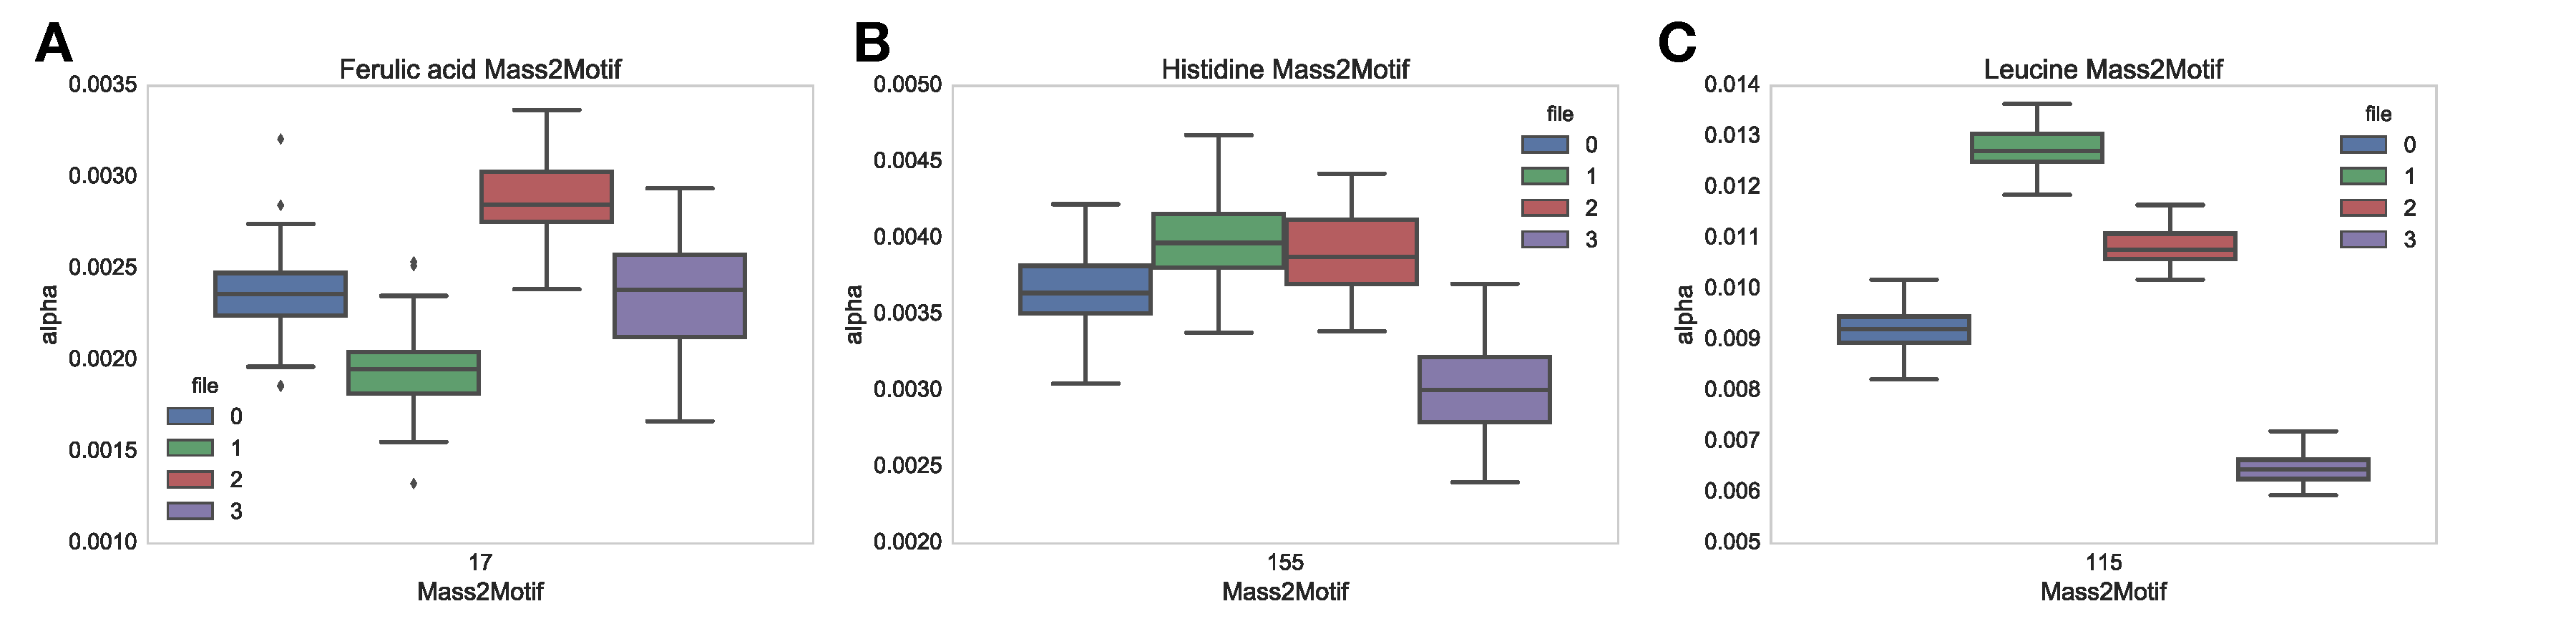
\includegraphics[width=1.0\linewidth]{07-lda/figures/multifile_alpha.pdf}
\centering\caption{Posterior alpha values for the \textbf{A)} ferulic acid, \textbf{B)} histidine and \textbf{C)} leucine Mass2Motifs across the different beer files. \label{fig:multifile-lda-alpha}}
\end{figure}

\section{Conclusion}

We have introduced MS2LDA, a pipeline that simplifies fragmentation data by exploiting the parallels between MS fragmentation data and text documents. The pipeline performs all steps required in the analysis: the preparation of a co-occurrence matrix of fragment and loss features in fragmentation spectra, the LDA analysis, and the graphical visualization of the resulting output. Evaluation of the workflow on beer extracts result in numerous informative patterns of concurrent mass fragmental and neutral loss, termed Mass2Motifs, which we could annotate as biochemically-relevant substructures. The MS2LDA approach is markedly different from other advanced spectral analysis tools as multiple Mass2Motifs can be associated with one metabolite, and determination of the key mass fragments or neutral losses that are part of a conserved structural motif is unsupervised. The application of LDA to modelling the fragmentation spectra produced by mass spectrometry instrument is exhaustively explored in this chapter. We have shown how spectra comprise of multiple substructures which can be explained by characterised Mass2Motifs. Through comparison to Molecular Networking, we demonstrated through examples how MS2LDA allows us to explain parts of a spectrum, producing a better functional annotation in contrast to spectral clustering where a spectrum can only be placed in one cluster. The differential analysis of parent ions having fragments sharing Mass2Motifs introduces the possibility of assessing changes in the expression levels of metabolites --- sharing substructures explained by a characterised Mass2Motif --- despite the identities of the metabolites unknown. This is particularly useful in the case of untargeted metabolomics experiments.

As future work, we envision developing a larger library of characterised Mass2Motifs from data sets produced on a diverse range of analytical platforms and different sample types. A challenge to this approach lies in the fact that mass spectrometry instruments have varying accuracy and therefore require different binning thresholds. One possible solution is define a common space of chemical vocabulary; rather than using binned fragment and loss features; a Mass2Motif can now be defined as the distribution over chemical formulae words. Such an approach is hampered by the fact that \textit{de novo} elemental formula assignment itself is a difficult problem, with large uncertainties as to the correctness of annotated formulae of a fragment or loss feature. A probabilistic model of formula annotation that can offers confidence values on the formulae annotation of a fragment or loss feature might be useful in this scenario as formula annotation uncertainties can then be incorporated into Mass2Motif formation in MS2LDA. Non-parametric model such as the Hierarchical Dirichlet Process \cite{Teh2006} can also be applied for topic discovery by letting the number of Mass2Motifs to be learned from the data itself. This allows for a truly flexible system of substructure annotation where Mass2Motifs can be obtained from training the model on large public fragmentation databases, such as HDMB or MassBank. In a similar manner as our analysis in this chapter, the resulting Mass2Motifs can be characterised. New and unseen fragmentation spectra can be run using the pre-trained models with these characterised Mass2Motifs, allowing for the rapid identification of the substructure that comprise a fragmentation spectra.

An extension of the standard LDA model, in form of the multi-file LDA model, is also proposed in this chapter to handle Mass2Motif inference from multiple data sets. Such a model can be used in large-scale clinical and metabolomic studies. In this model, the prior information on which prior Mass2Motifs the user expects to see can be included into the MS2LDA workflow, allowing the LDA inference on certain known Mass2Motifs that are expected to be present in the sample while allowing others to be inferred from the data.

Other LDA-based techniques developed for text (e.g. hierarchical LDA \cite{griffiths2004hierarchical}) are also likely to offer benefits as we hypothesise that Mass2Motifs can be defined in a hierarchy. For instance, generic patterns such as the loss of CO2 may lie at the top of the hierarchy of Mass2Motifs, while the more specific Mass2Motifs are formed at the bottom. It is anticipated that visualisation and the meaningful presentation of inference results will be a challenging task in such a model. 

In general, we anticipate that the approach of applying topic modelling techniques to fragmentation spectra data to be particularly useful in research areas such as clinical metabolomics, pharmacometabolomics, environmental analysis, natural products research and nutritional metabolomics, as it can quickly and in an unsupervised manner recognize substructure patterns related to drugs, pollutants, and food-derived molecules, respectively. 